% !TeX spellcheck = en-US
% !TeX encoding = UTF-8
% !TeX root = ../thesis.tex

\chapter{Evaluation}
\label{ch:Evaluation}
% pages: 7.14-9.52

This section elaborates on the results of our experiments. As a proof of concept, we aimed to show, that our architecture is able to learn rendezvous tasks with a more or less GNN Blocks (1). Then we compared training on a set of agents, while evaluating on a different number of agents (2). Afterwards we showed the effect of different aggregation functions on training (3), and how multiple GNN hops can affect the result if the observation radius for the agent varies (4). 
%\begin{itemize}[noitemsep,nolistsep]
%    \item (1001-7-pursuit-multi-neighaggr)
%    \item (1001-8-directed-vs-undirected-graph)
%    \item (1001-9-value-nodewise-graphwise)
%\end{itemize} 
\par

Evaluation of the results used different environments compared to training. While the agents trained on randomized starting positions, they were tested with fixed starting positions to allow comparable results. A similar setting was used for evader starting position in Pursuit environments. We considered the average reward per training step and the last reward per training step as performance metrics. The mean gave us a meaningful metric for the progress of the RL algorithm, while the last reward had a more geometric importance for solving the tasks like Rendezvous.  \par

A more detailed overview of the PPO parameters we use can be found as an appendix \Cref{ch:Hyperparameters}. Unless mentioned otherwise, the following experimental settings were used:
\begin{itemize}[noitemsep,nolistsep]
    \item The plots show the standard error from the input data.
    \item The environment always used a torus setup (position is wrapped using modulo, no borders).
    \item Observations did not directly include the positions of agents or evaders which would trivialize the tasks.
    \item No observation culling was used: Each agent could see every other agent and evader.
    \item The agents used direct dynamics: Their actions directly influenced movement on the x- and y-Axis.
    \item Rewards and Observation were normalized using a running mean and std to improve learning.
    \item Used mean aggregation.
    \item Independet GNN-stack for the actor and critic, which used residual connections.
\end{itemize} \par

During the evaluation of the experiments, we experienced unexpected hardware issues that caused a subset of our runs to crash. Due to time constraints, we were not able to fully replicate the respective experiments. Note that we do not include these crashed runs in our evaluation, and that the resulting grid searches are thus partially incomplete. The general findings of this thesis remain unchanged. \par



\section{Proof of Concept}
\label{sec:Proof of Concept}
% ~ 1 page
This proof-of-concept experiment used rendezvous. We wanted to show that our architecture works in general. Furthermore, we wanted to investigate if multiple can already have an impact on learning for rendezvous without any observation culling. We chose to use 10 agents that have 24 timesteps to meet each other in a torus-world of size 12. For these runs we used latent dimension in the range of 8 to 64 and 1 to 4 number of hops. The last reward of a given iteration tells us if the agents were able to meet up in the allotted time and therefore we choose that as a comparison.

\begin{figure}[htp]
    \centering
    \subfigure[Number of Hops]{\label{fig:proof_of_concept_rendezvous_1}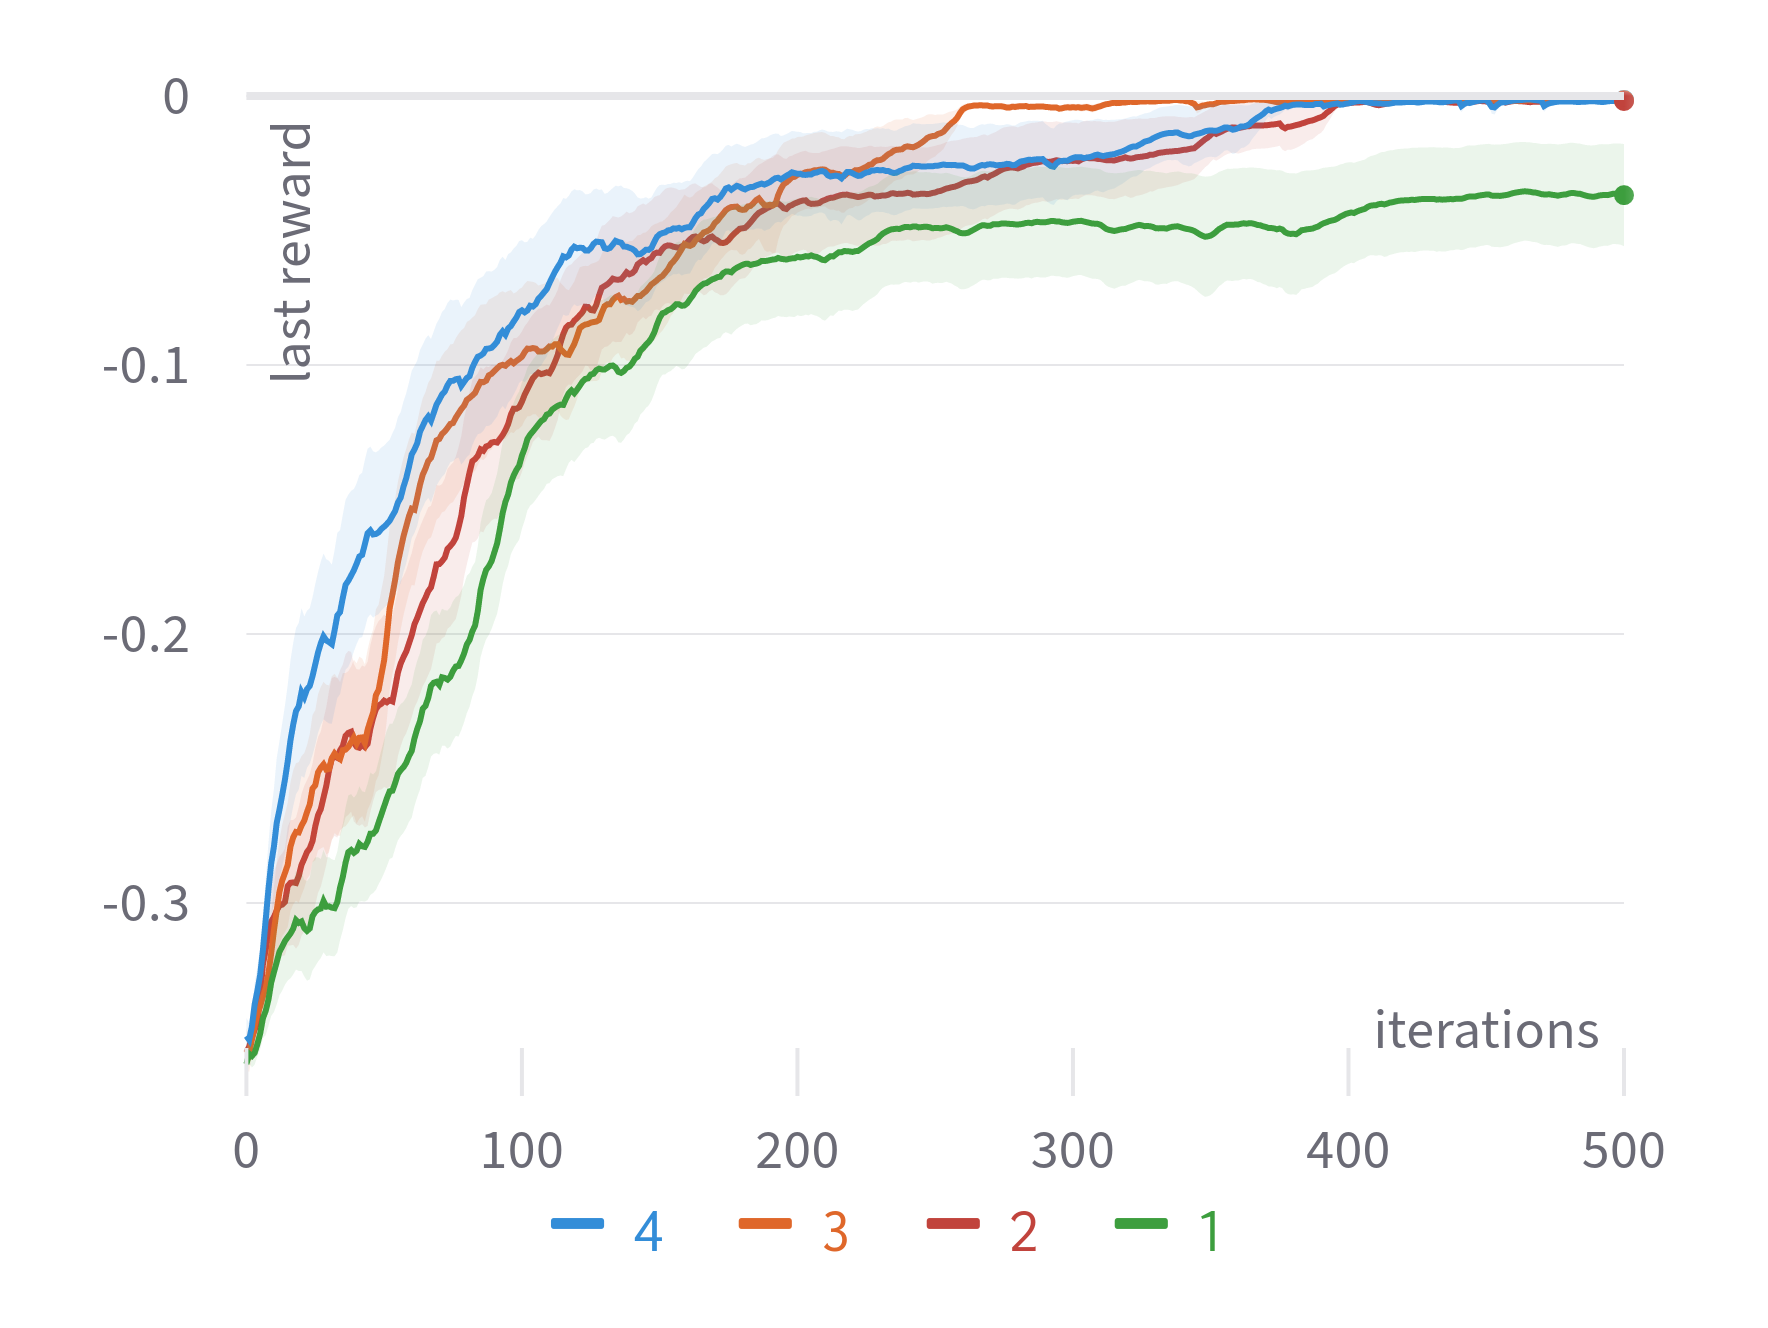
\includegraphics[width=0.49\textwidth]{figures/proof_of_concept_rendezvous_1.png}}  
    \subfigure[Latent Dimension]{\label{fig:proof_of_concept_rendezvous_2}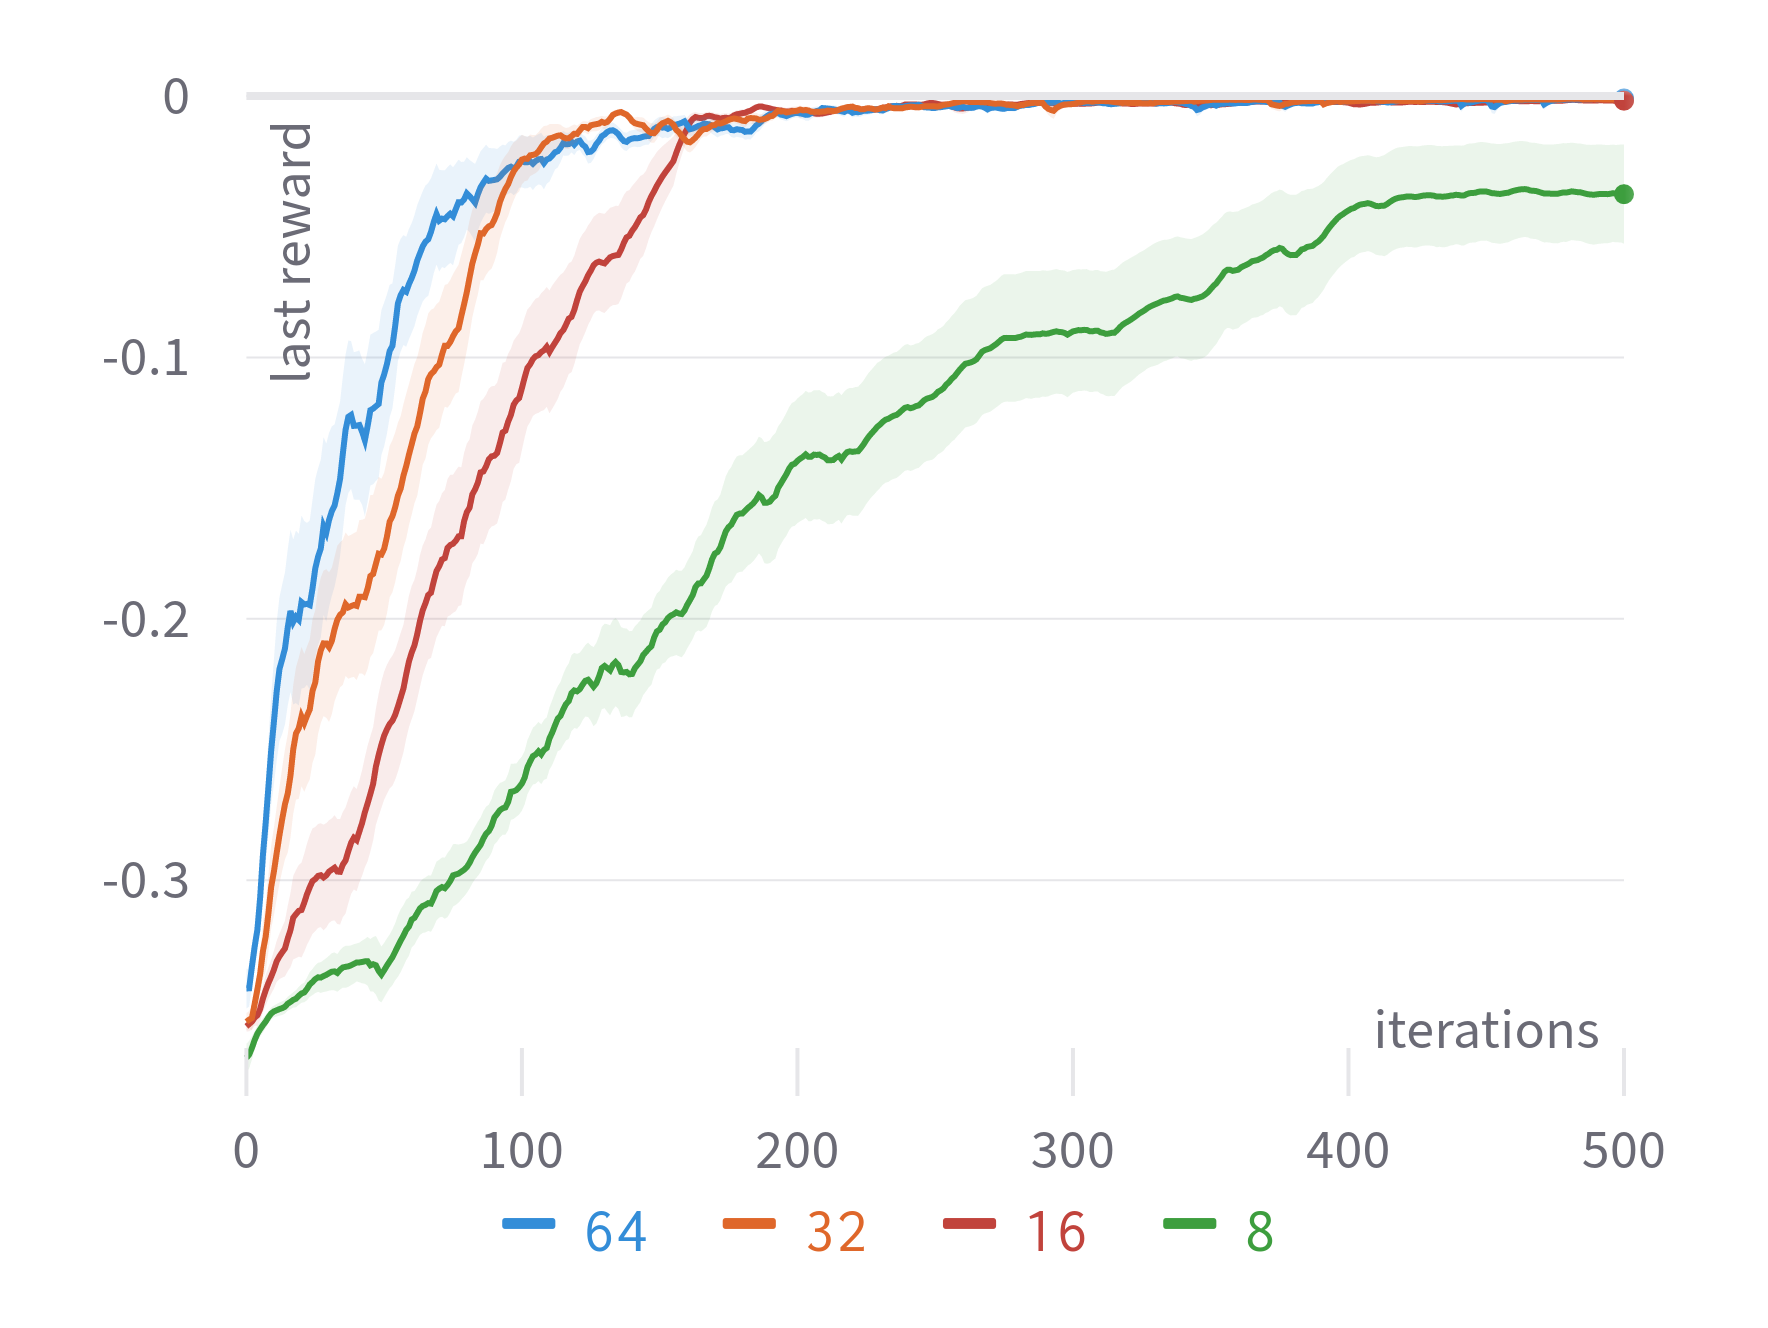
\includegraphics[width=0.49\textwidth]{figures/proof_of_concept_rendezvous_2.png}}  
    \hspace{1cm}                       
    \caption{Results of the Rendezvous task for different latent dimensions. The left side shows the different number of hops, while the right side shows different latent dimensions.}
    \label{fig:proof_of_concept_rendezvous}
\end{figure}

\Cref{fig:proof_of_concept_rendezvous} clearly shows that most of the training environments were able to successfully solve the task. With at least 2 hops, the task was solved, and no extra benefit can be seen for more than 2 hops. Earlier in training, the performance shows some difference for more hops. It is clear that the architecture is able effect the observation input more strongly and learn faster. Each extra hop added roughly 13$\%$ to the time needed to learn, so the benefit is rather small. For simple task, this was expected. If we look at the right site, we can see the effect of different latent dimension to the effectiveness of learning. Only a latent dimension of 8 was not enough for the agents to meet up in the allotted time. In that case, it is clear that the architecture was not able to correctly represent and process observation data for 10 agents.\par

\begin{figure}[htp]
    \centering
    \subfigure[Latent Dimension: 8]{\label{fig:proof_of_concept_rendezvous_ld8}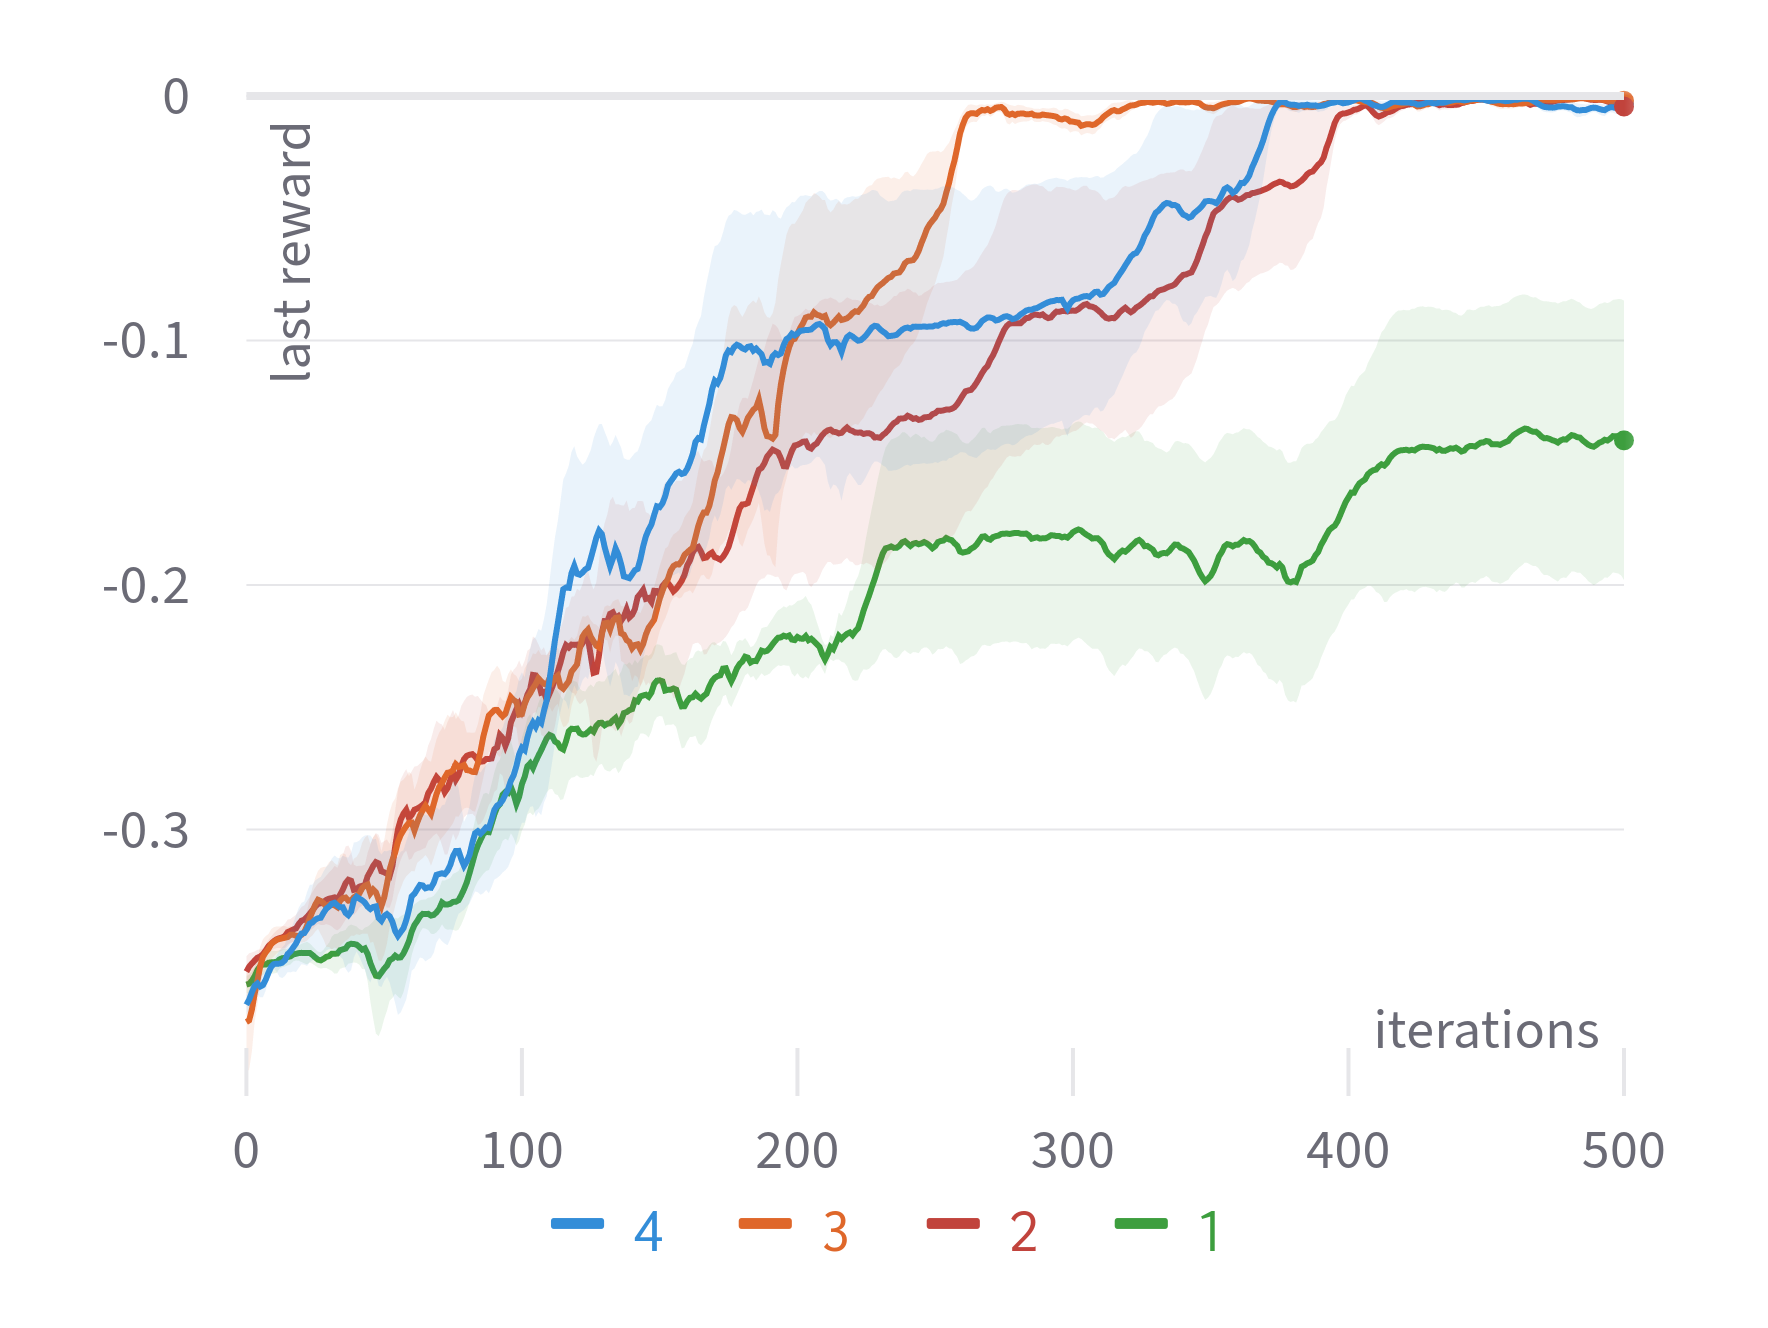
\includegraphics[width=0.49\textwidth]{figures/proof_of_concept_rendezvous_ld8.png}}  
    \subfigure[Latent Dimension: 16]{\label{fig:proof_of_concept_rendezvous_ld16}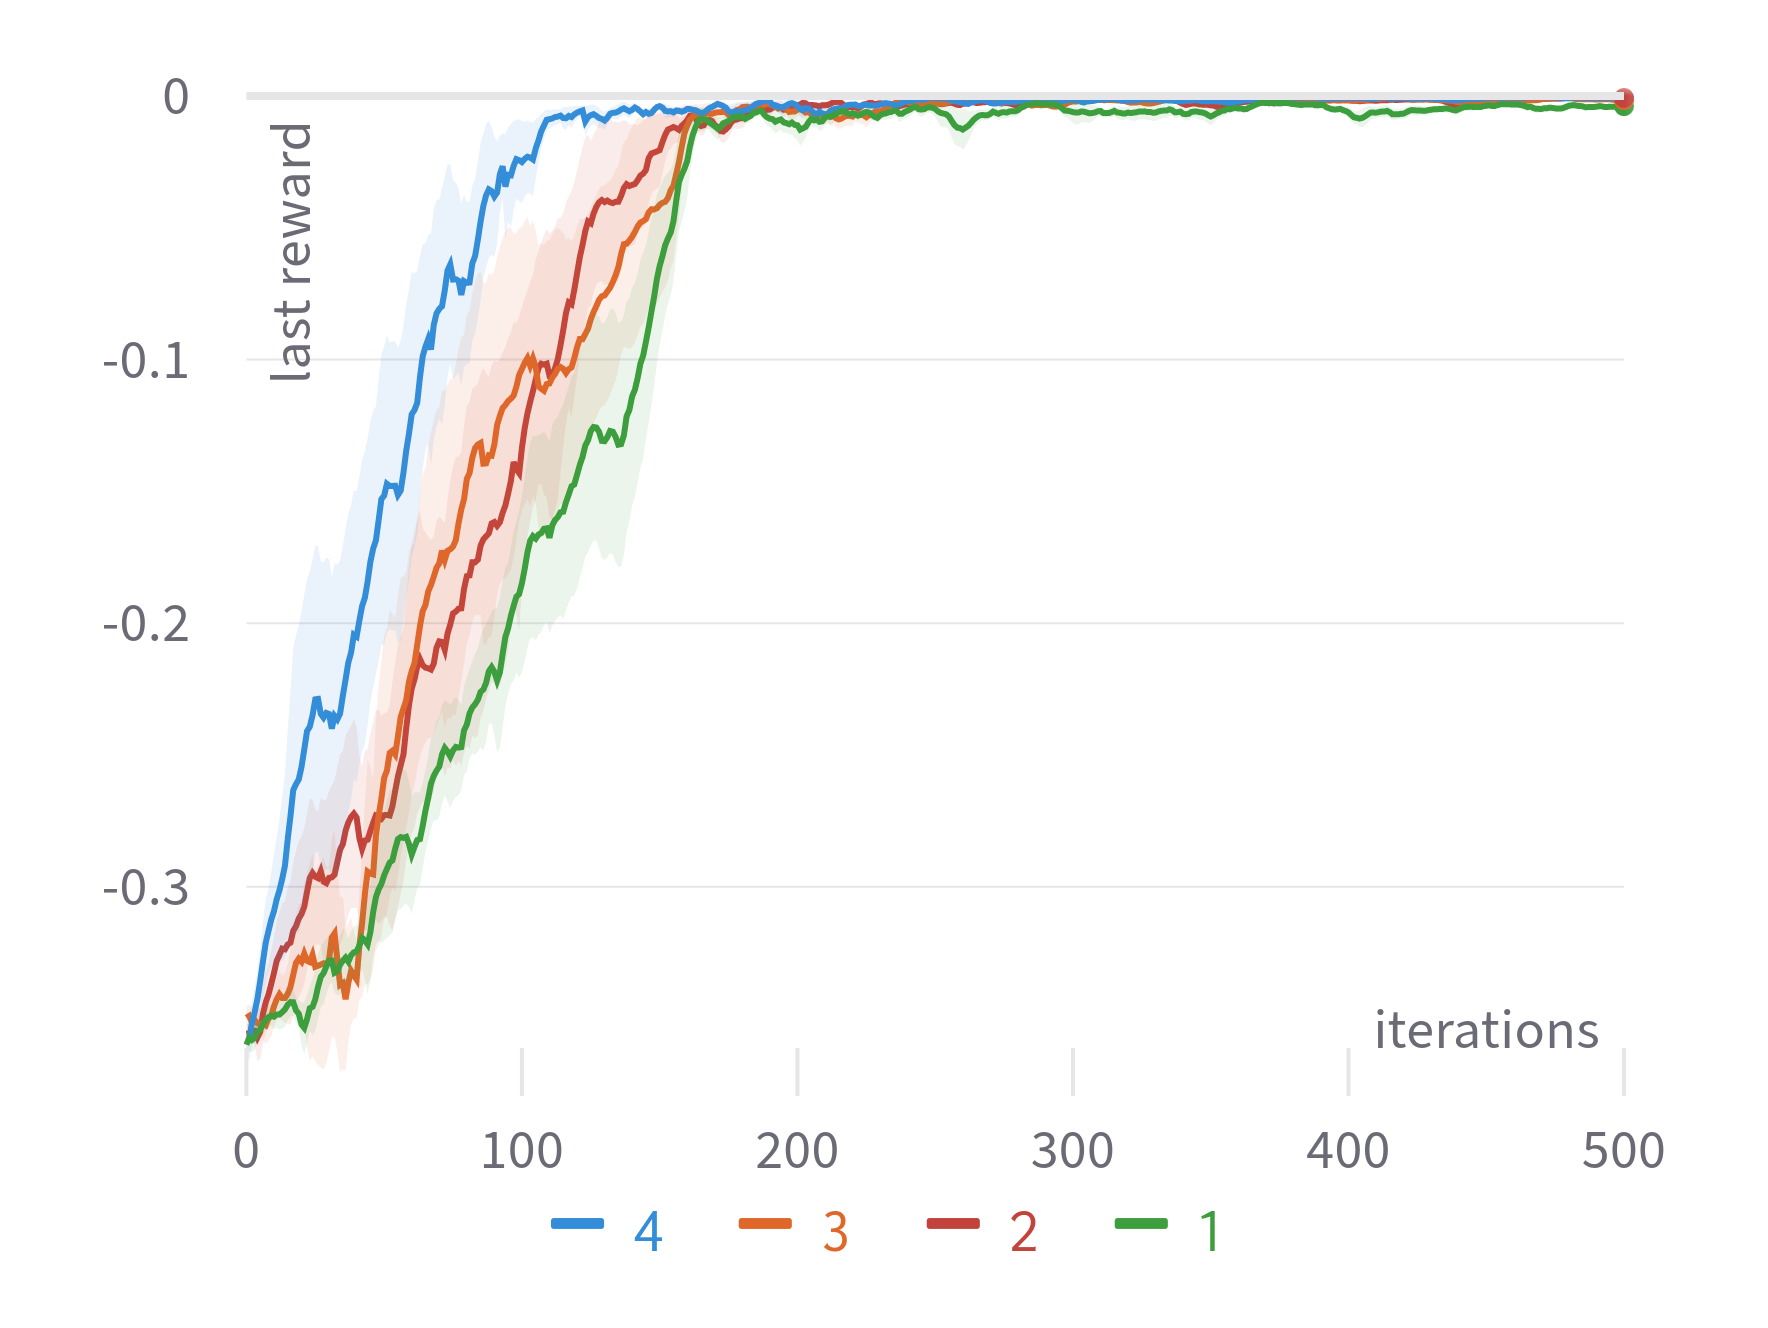
\includegraphics[width=0.49\textwidth]{figures/proof_of_concept_rendezvous_ld16.png}}  
    \hspace{1cm}                       
    \caption{Here we filtered the results for a latent dimension of 8 on the left and 16 on the right.}
    \label{fig:proof_of_concept_rendezvous_ld}
\end{figure}

If we investigate the behavior for the different latent dimensions, we can see a large difference in performance shown in \Cref{fig:proof_of_concept_rendezvous_ld}. For a latent dimension of at least 16 the difference between the number of hops is quite small, as can be seen on the right side. If we filter the results for a latent dimension of 8, the general performance is expectedly worse. But the difference between the number of GNN hops is much more pronounced. This shows that, in larger constraints, the ability to process more of the observation data leads to a larger gain. As doubling the latent dimension also roughly doubles the total time needed, we conclude that more hops can be more efficient than a higher latent dimension.


\section{Ablation}
\label{sec:Ablation}
% ~ 1 page
In these experiments we want to examine how good our architecture was in ablation tests. In other words, how good the it would be able to abstract the task at hand while using a different amount of agents to train than to evaluate. Overall, we chose to use the same number of timesteps and same torus-size then the proof of concept. We used a latent dimension in the range of 8 to 32 and 1 to 4 number of hops. We trained on 5,10, or 20 agents and evaluated on 5,10, or 20 agents.

\begin{figure}[htp]
    \centering
    \subfigure[Training: 5 Agents, Evaluation: 20 Agents]{\label{fig:ablation-5-to-20}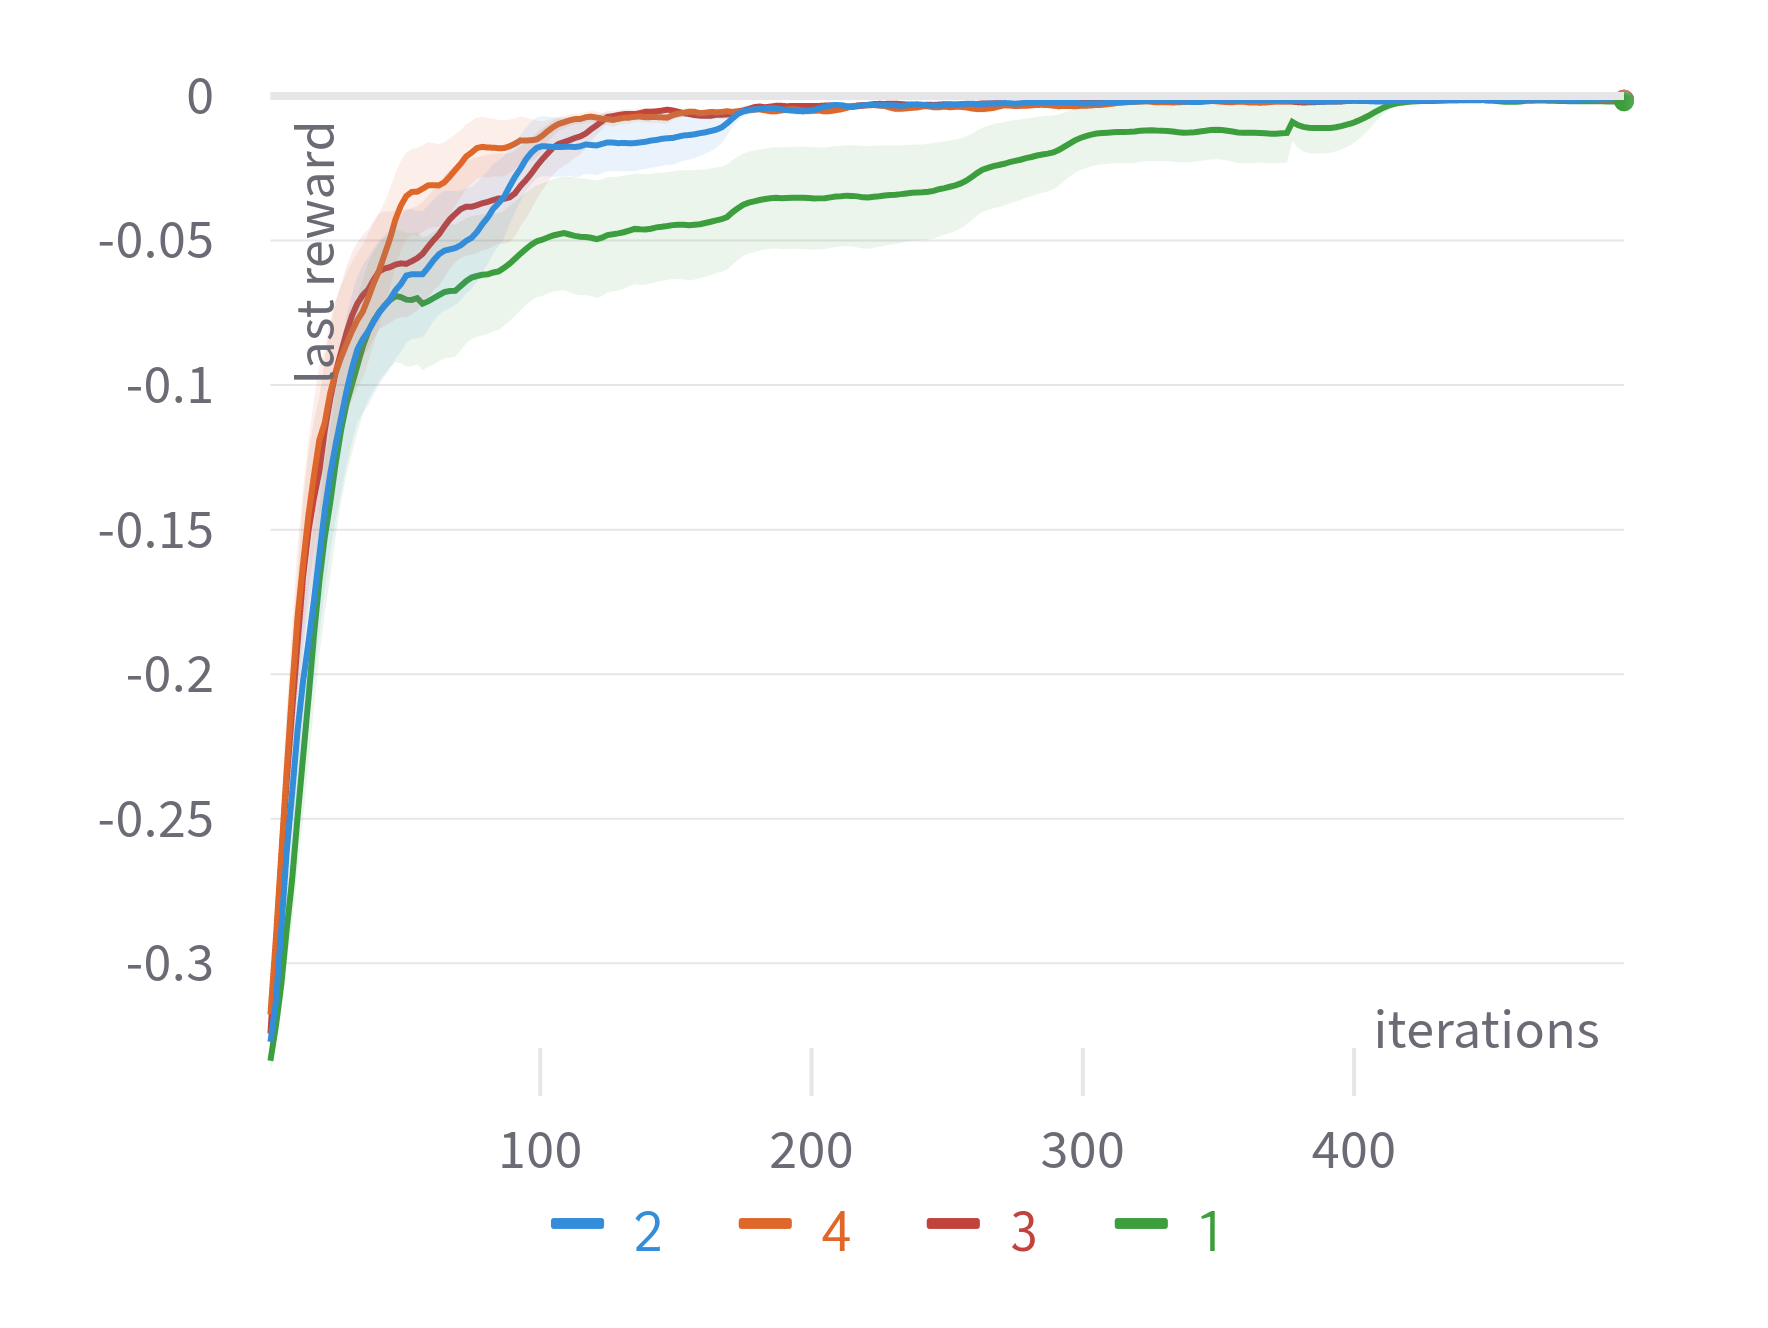
\includegraphics[width=0.49\textwidth]{figures/Ablation_5-to-20.png}}  
    \subfigure[Training: 20 Agents, Evaluation: 5 Agents]{\label{fig:ablation-20-to-5}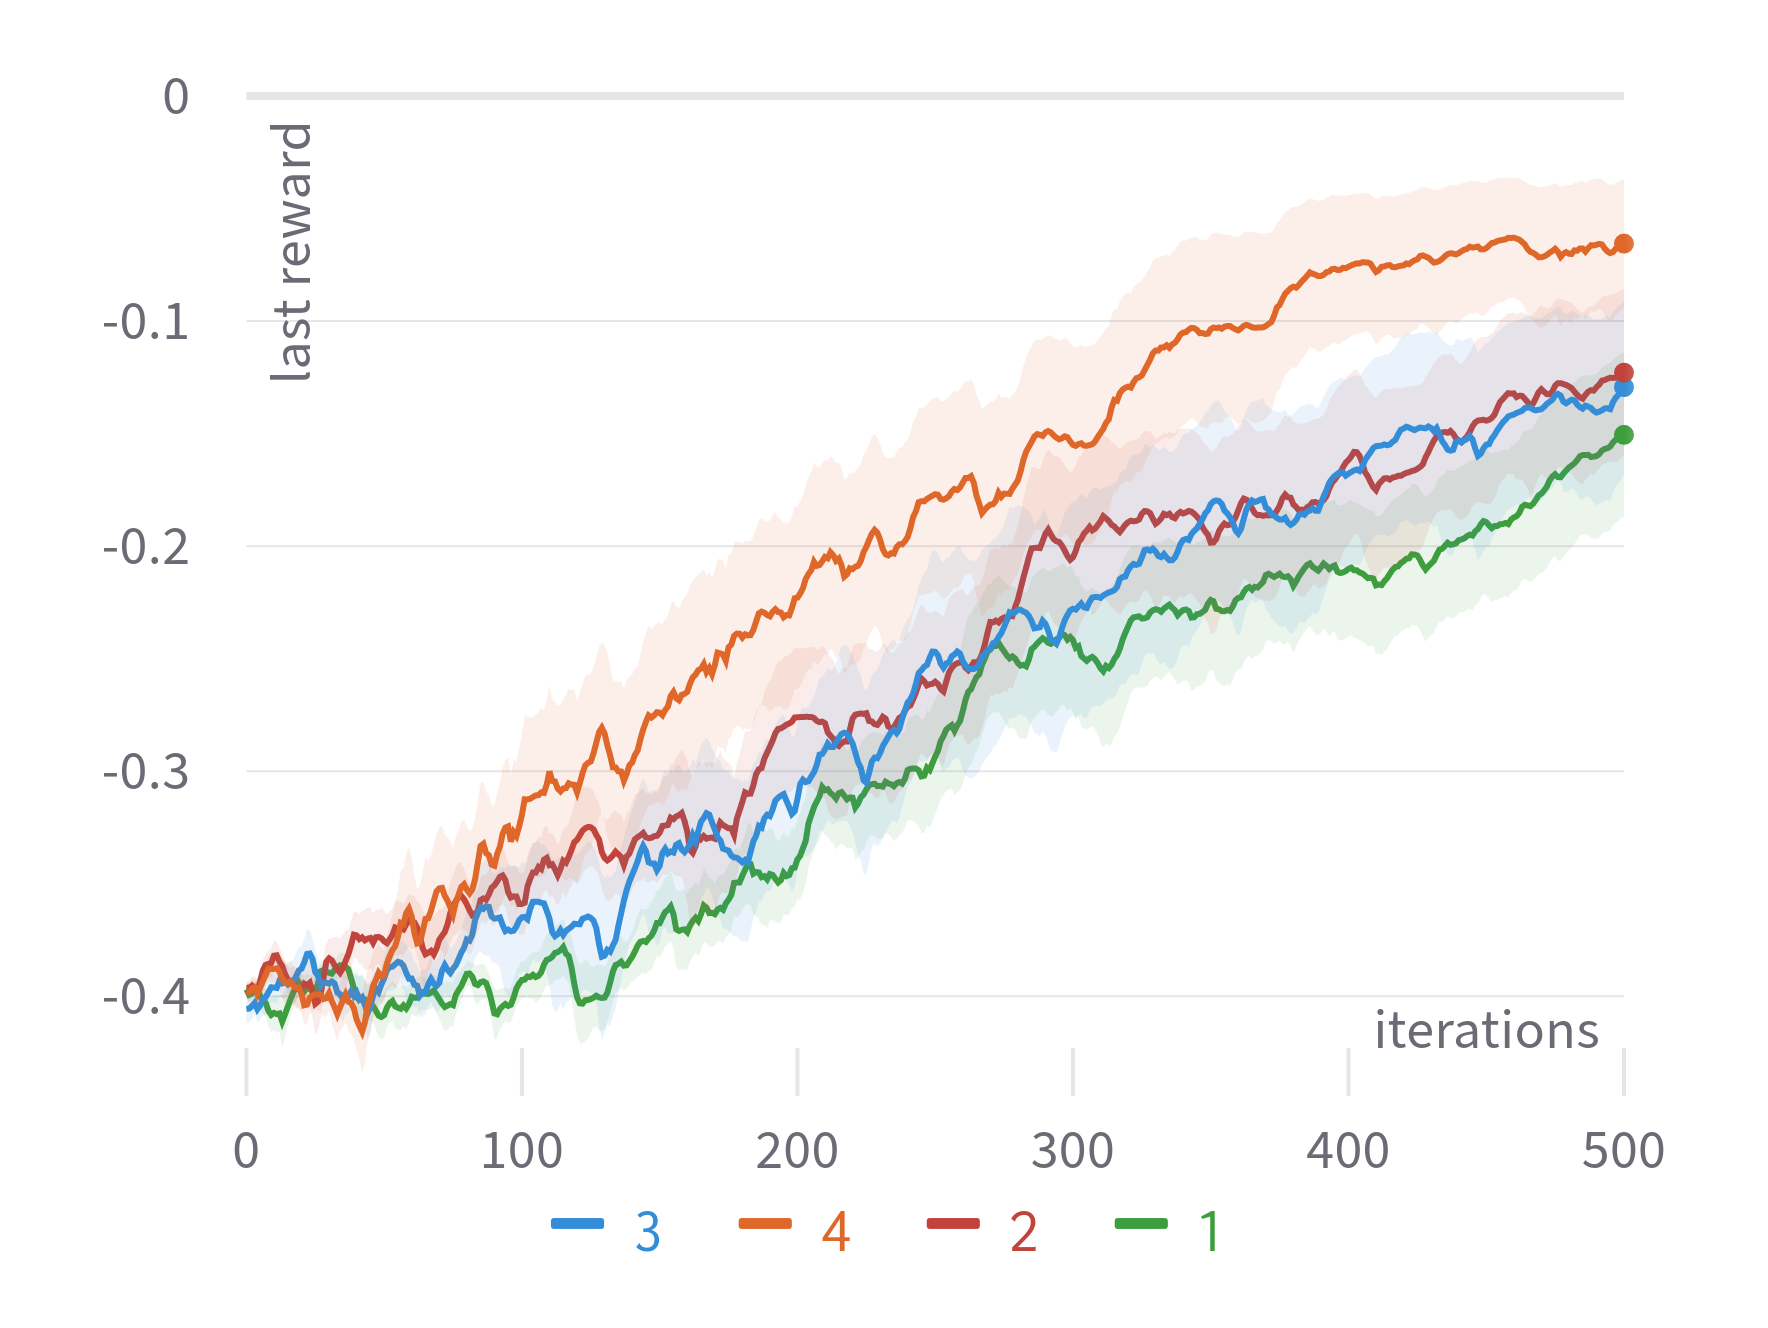
\includegraphics[width=0.49\textwidth]{figures/Ablation-20-to-5.png}}  
    \hspace{1cm}                       
    \caption{Performance of different amount of GNN hops for ablation. The leftside shows successfull training with 5 agents and evaluation with 20 agents. Training with 20 agents was more difficult}
    \label{fig:ablation-5-20-20-5}
\end{figure}

\Cref{fig:ablation-5-20-20-5} examines the two extreme cases of our ablation test. We did not feature learning on 10 agents, as it did not prove any results. On the left side we see no discernable difference between 2 to 4 GNN Hops. All of them were able to solve the task in roughly the same time. A single hop is shown as an outlier which performed considerably worse. It took more than double the time to solve the task. No real benefit for more than a single hop can be found for an upwards ablation. The right side shows the downward ablation of 20 training agents and 5 evaluation agents. Given that this is a harder task to learn, we can clearly see that the solutions still led to a gap between the agents. Though noisy, 2-3 hops performed better overall than a single hop. However, a sizeable difference for 4 hops can be observed. This holds true if we filter the results for 20 training agents and 20 evaluation agents. This might indicate that the architecture with more hops is better suited for larger amounts of agents. 

\begin{figure}[htp]
    \centering
    \subfigure[Latent Dimension]{\label{fig:ablation-ld}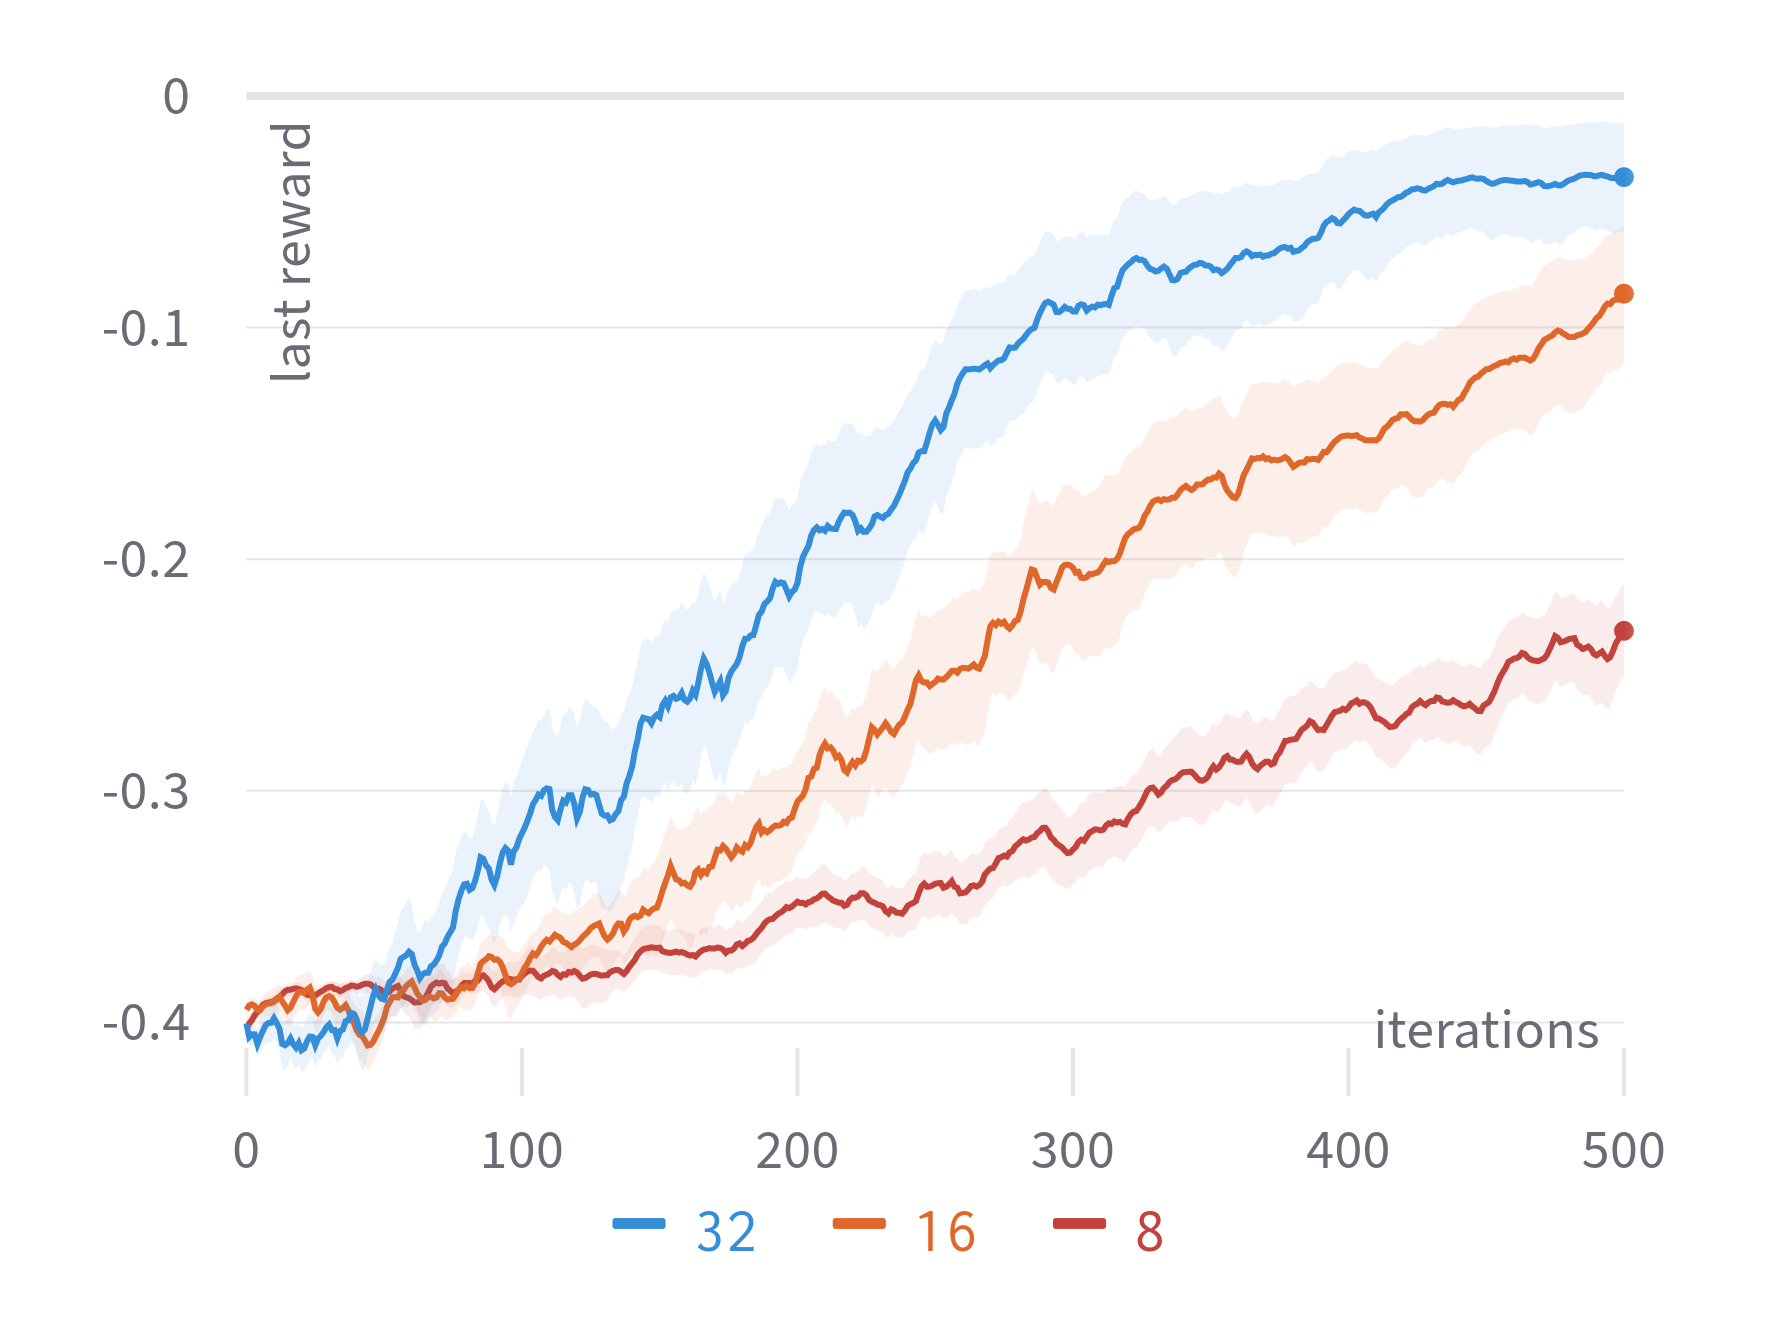
\includegraphics[width=0.49\textwidth]{figures/Ablation-ld.png}}  
    \subfigure[Number of Hops without Latent Dimension 8]{\label{fig:ablation-no ld8}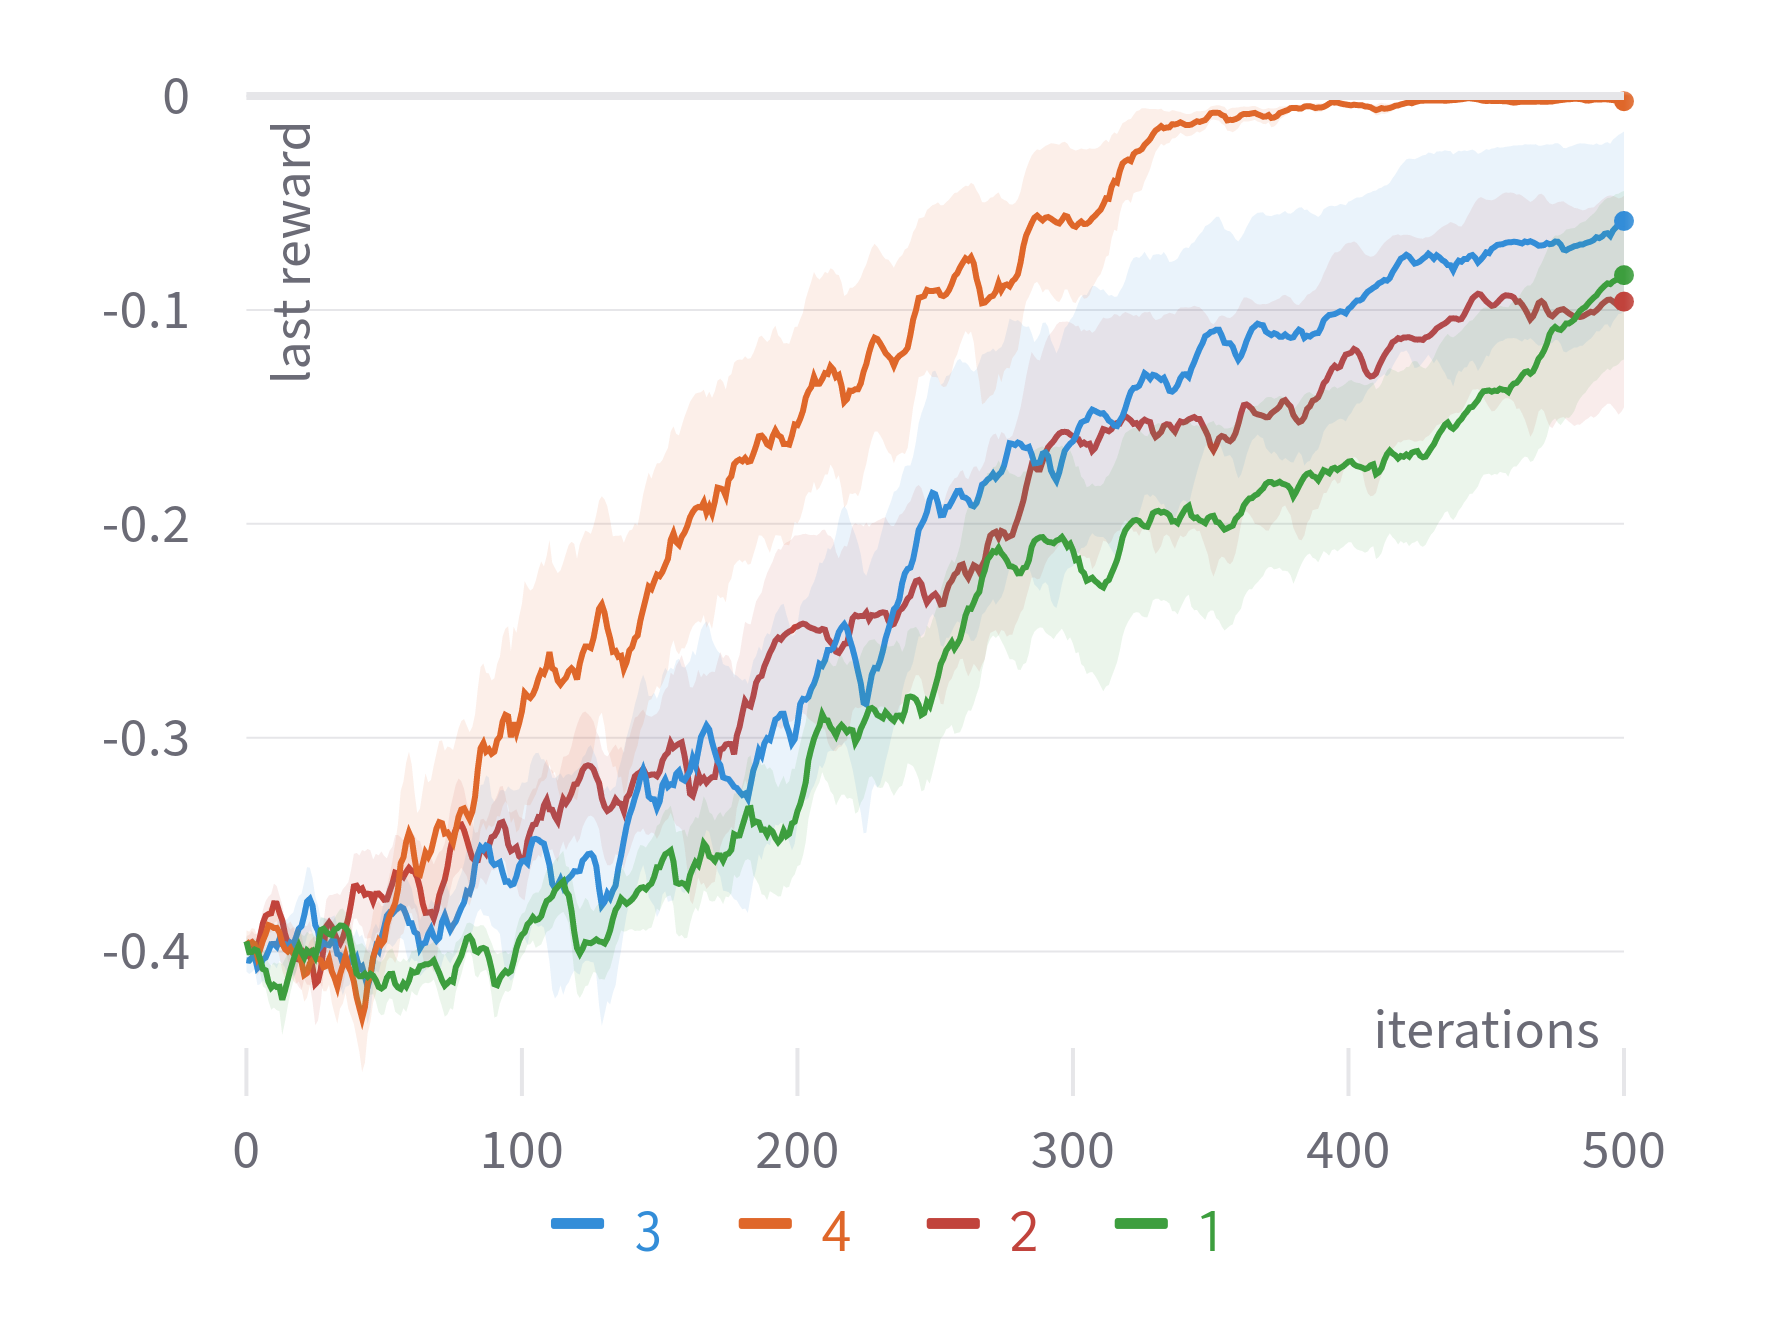
\includegraphics[width=0.49\textwidth]{figures/Ablation-no ld8.png}}  
    \hspace{1cm}                       
    \caption{Looking at the performance for the latent dimension shows a larger difference in the results on the leftside. Filtering out latent dimension of 8 shows a much stronger performance for 4 hops.}
    \label{fig:ablation-ld-no-ld8}
\end{figure}

We wanted to examine the results for 20 training agents and 5 learning agents a bit more. If we take a look at the performance of different latent dimensions on the left side of \Cref{fig:ablation-ld-no-ld8}, again we are able to that a latent dimension of 8 clearly lags behind. Filtering for latent dimension 8, which is not shown here, shows us very similar results to \Cref{fig:proof_of_concept_rendezvous_ld} in the proof of concept experiments. Because of this, we wanted to exclude latent dimension of 8 in the results. The right side clearly demonstrates a more pronounced difference for 4 GNN hops. It is the only setup that was able to solve the task. With a singular constraint, the downsizing of information gathered by agents and the resulting information sparseness, the results were much more pronounced.


\section{Different Aggregation Functions}
\label{sec:Different Aggregation Functions}
For these experiments we looked at the dispersion environment and different aggregation functions used by the architecture. The goal was to examine the effect of aggregation functions to the learning effectiveness under different reward types. Dispersion used very similar parameters to Rendezvous. We used a latent dimension in the range of 8 to 32 and 1 to 3 number of hops.


\begin{figure}[htp]
    \centering
    \subfigure[Different Rewardtypes]{\label{fig:aggregation-rt}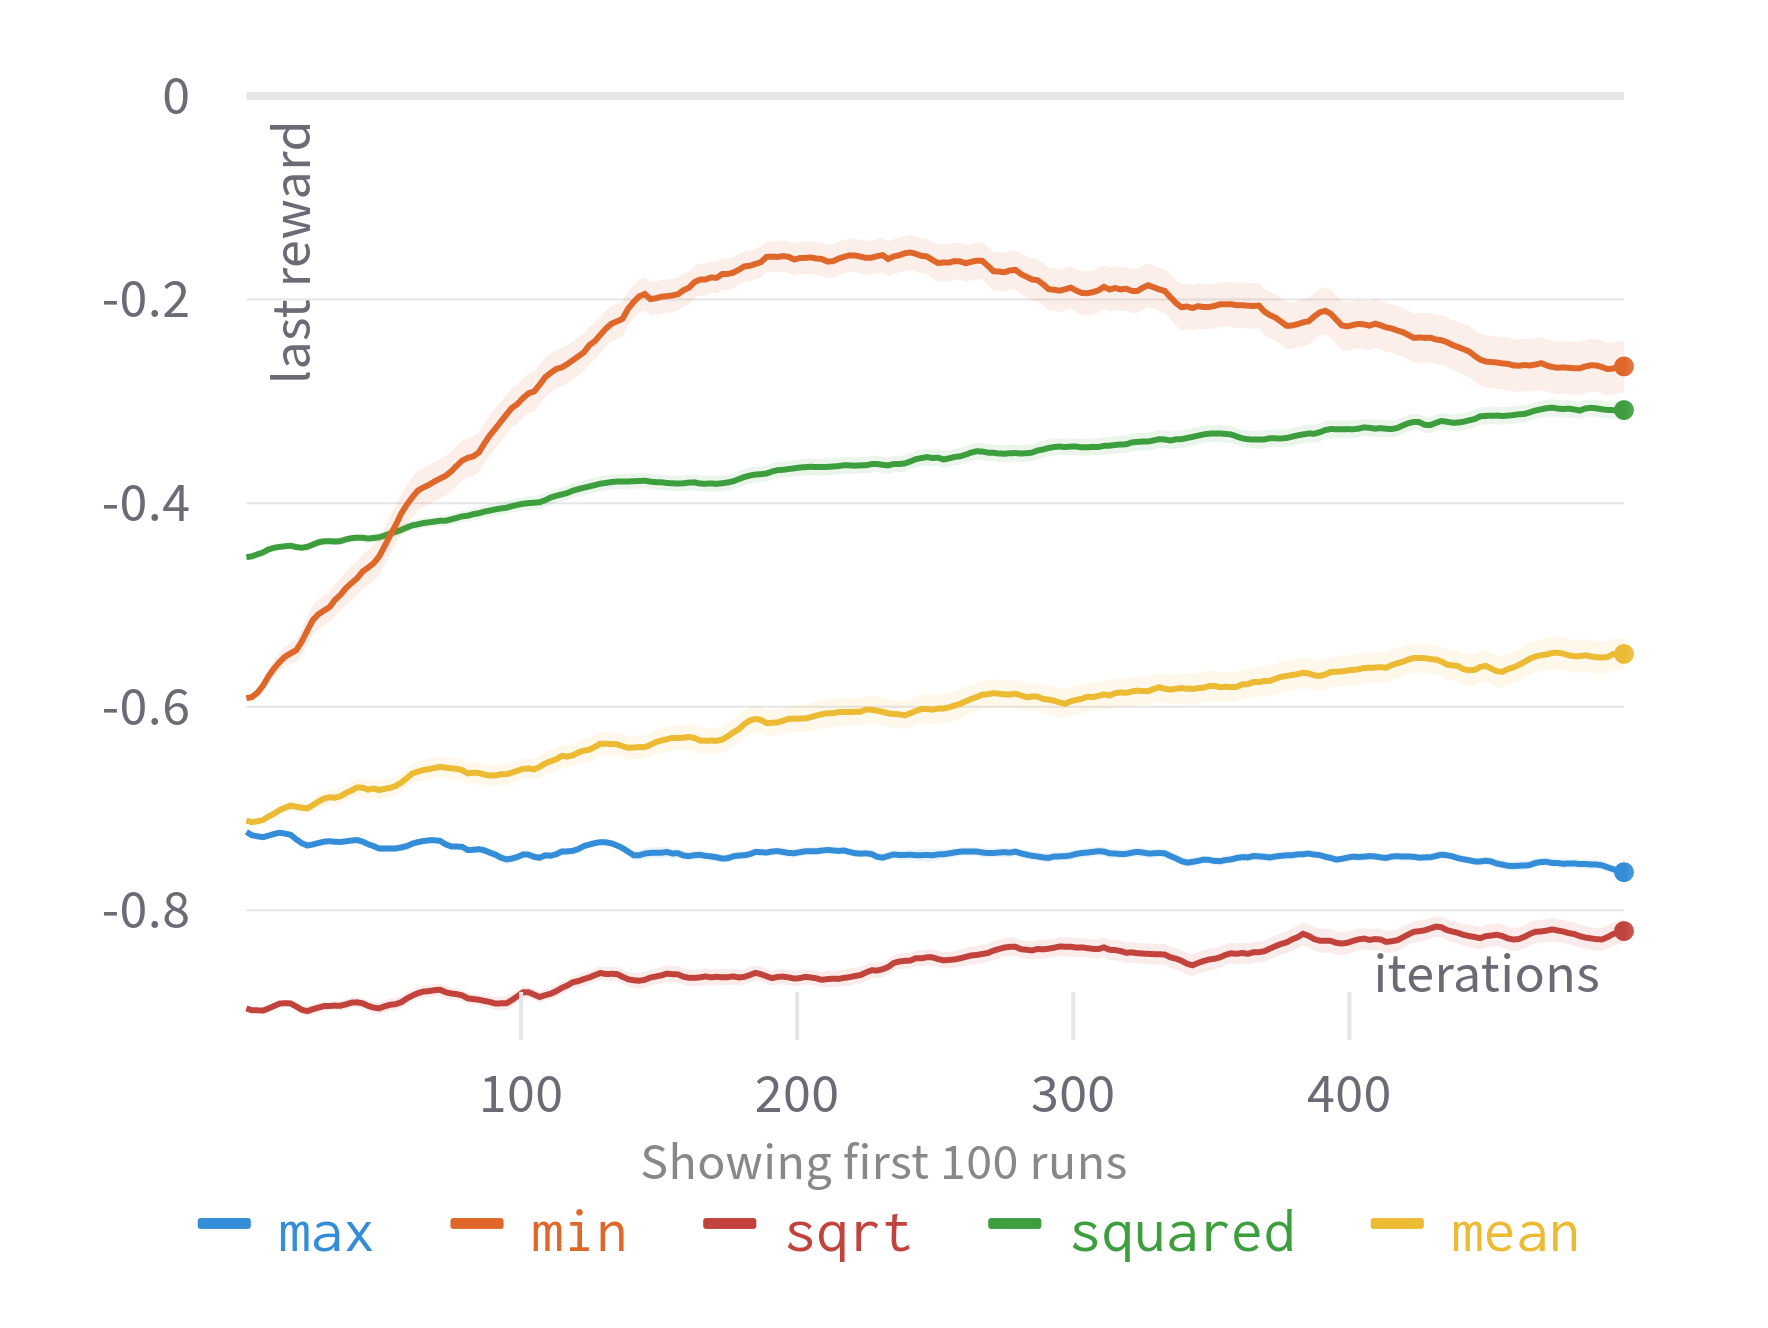
\includegraphics[width=0.49\textwidth]{figures/aggregation_rt.png}}  
    \subfigure[Different Number of Hops]{\label{fig:aggregation-nb}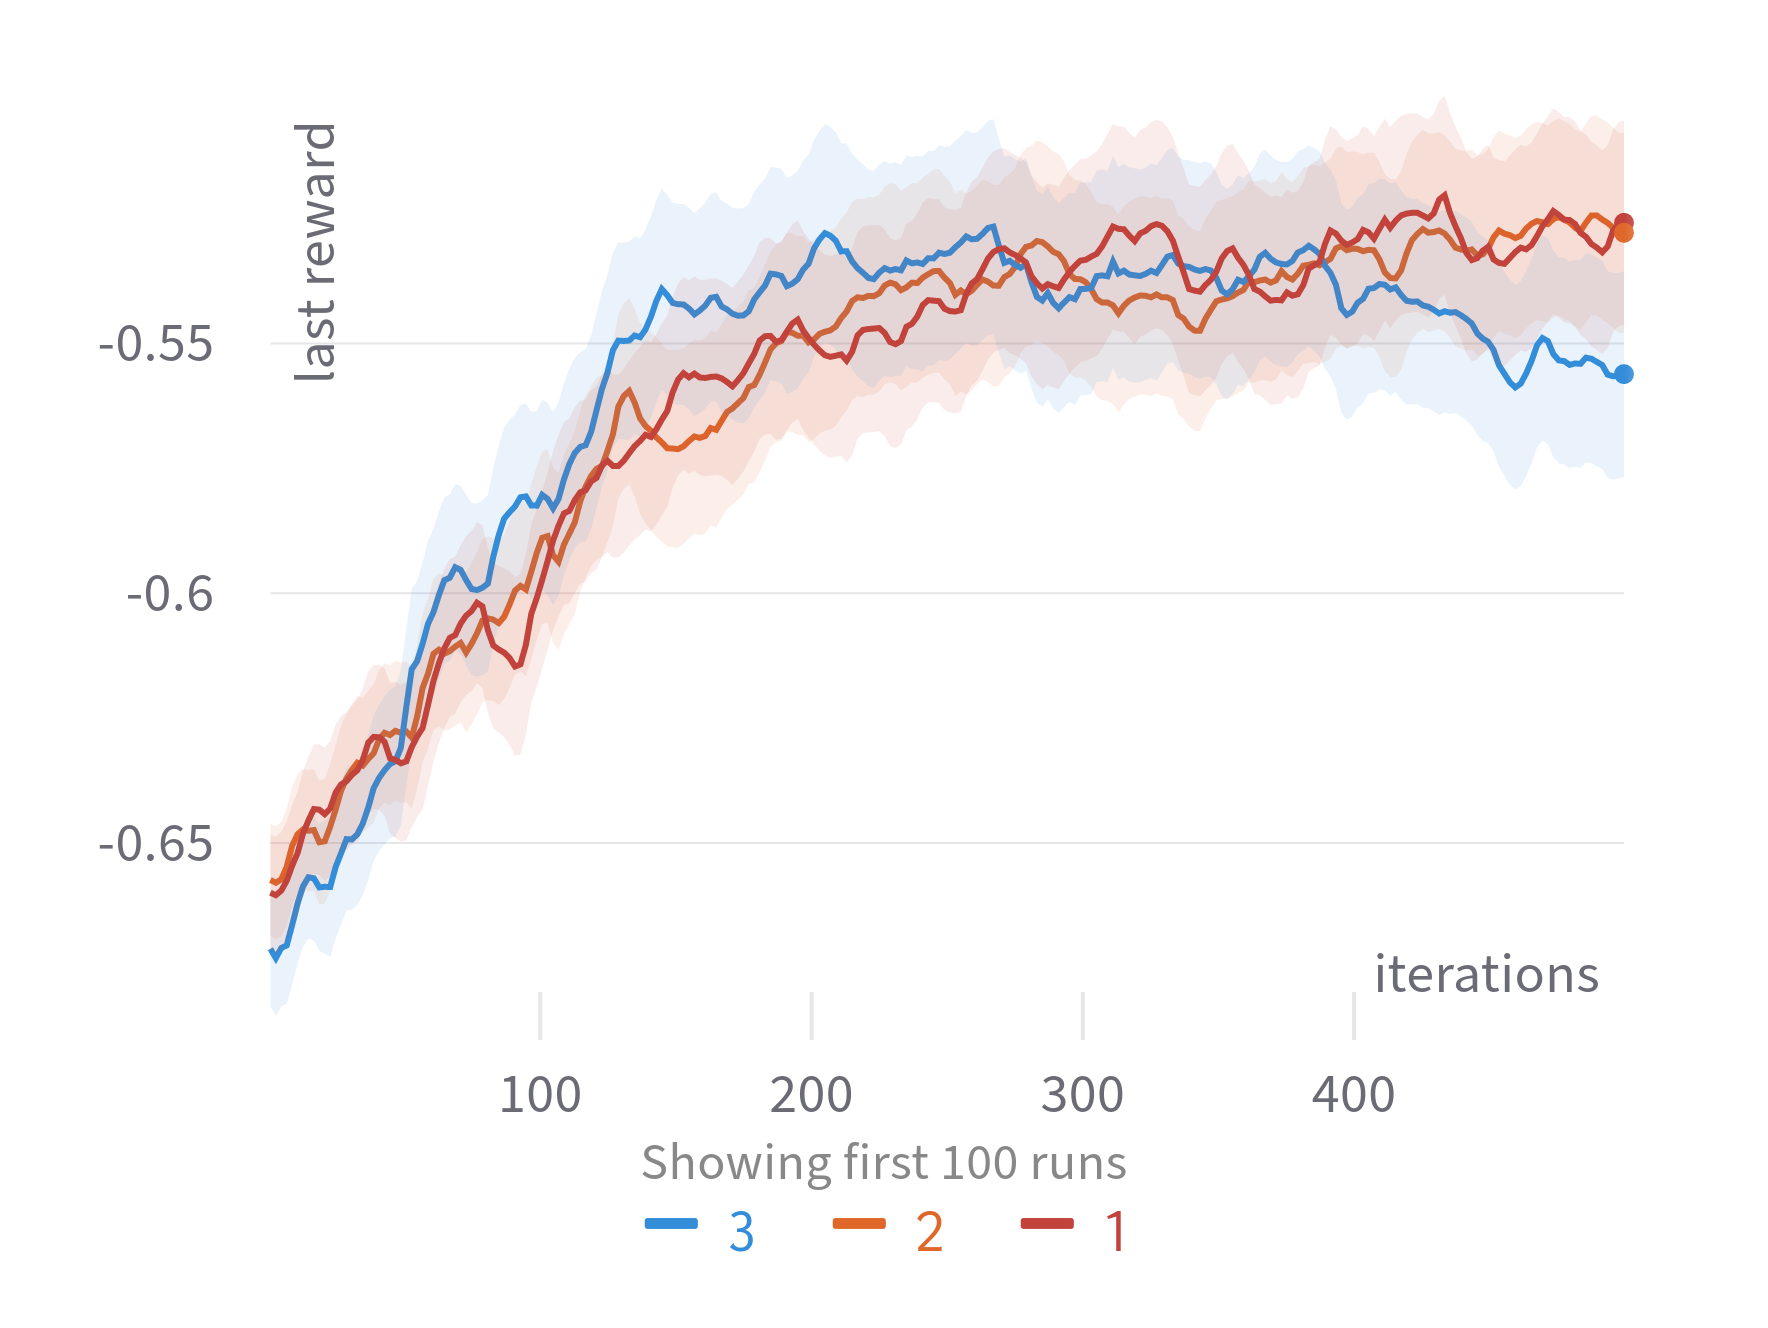
\includegraphics[width=0.49\textwidth]{figures/aggregation_nb.png}}  
    \hspace{1cm}                       
    \caption{Performance of different aggregation functions for the Dispersion task}
    \label{fig:aggregation-compare}
\end{figure}

\Cref{fig:aggregation-compare} shows our results for dispersion. We can generally see that the architecture was not able to learn for reward types mean, min and max. Furthermore, it shows that the number of hops did not make any difference in learning. If we filter for the different aggregation functions, we either observed no difference in the number of hops, or the setup did not learn at all. If we filter out mean, min and max, the results show no difference. This suggests that dispersion is either an outlier, not properly implemented, or shows that the GNN hops may not help in certain tasks. 


\section{Under Observation Constraints}
\label{sec:Under Observation Constraints}
% ~ 1 page
The goal for these experiments was to determine if the GNN hops had a larger impact when we use a limited observation range for our agents. For this we looked at kNN and Euclidean distance culling of 50, 25 and 12.5$\%$ respectively. In the case of Euclidean distance, the percentage is relative to the world size. For kNN it denotes how many agents of the total are visible. Tests were run from 8 to 64 latent dimension and 1 to 4 GNN hops.

\begin{figure}[htp]
    \centering
    \subfigure[kNN]{\label{fig:observation-knn}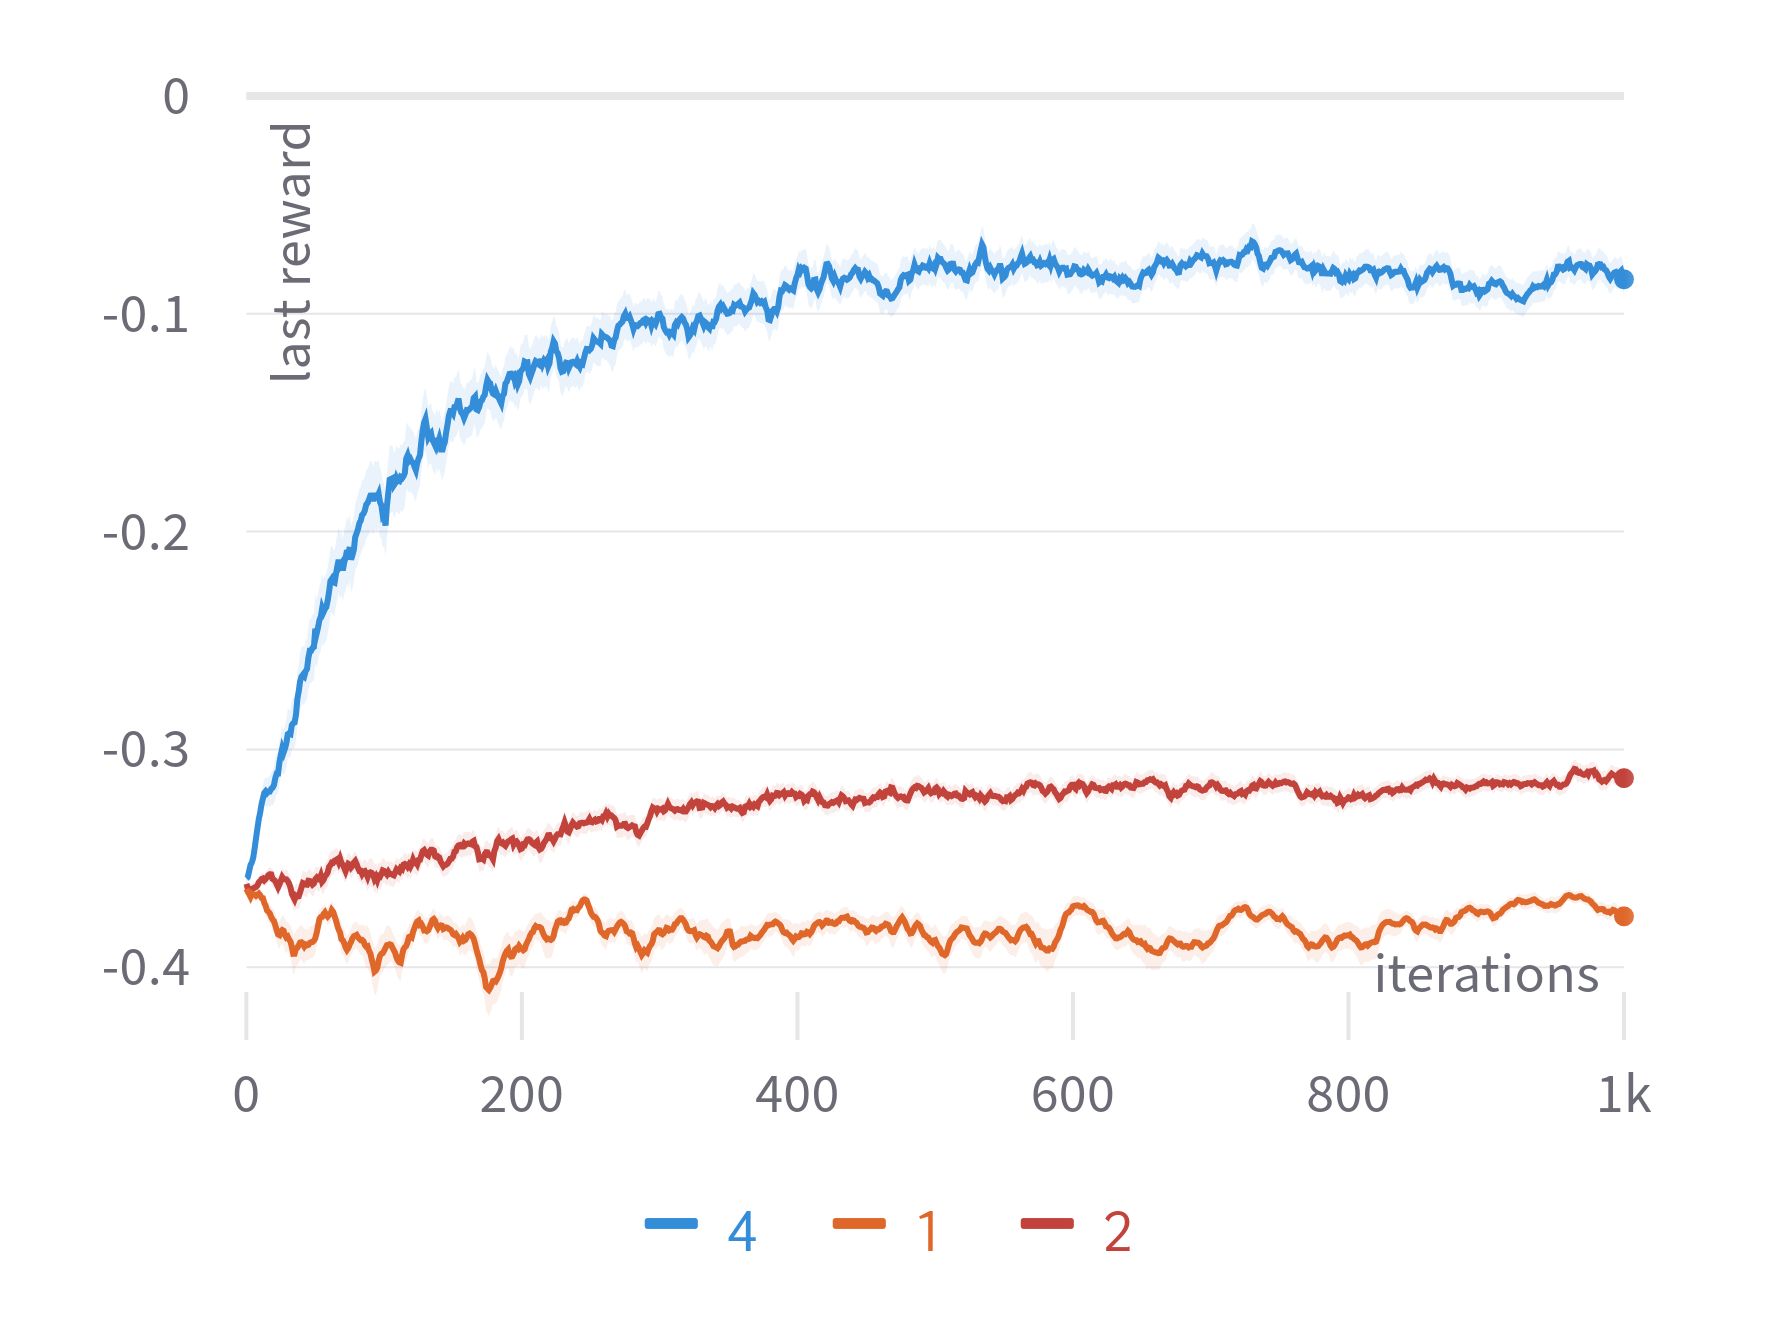
\includegraphics[width=0.49\textwidth]{figures/observation_knn.png}}  
    \subfigure[Euclidean Distance]{\label{fig:observation-distance}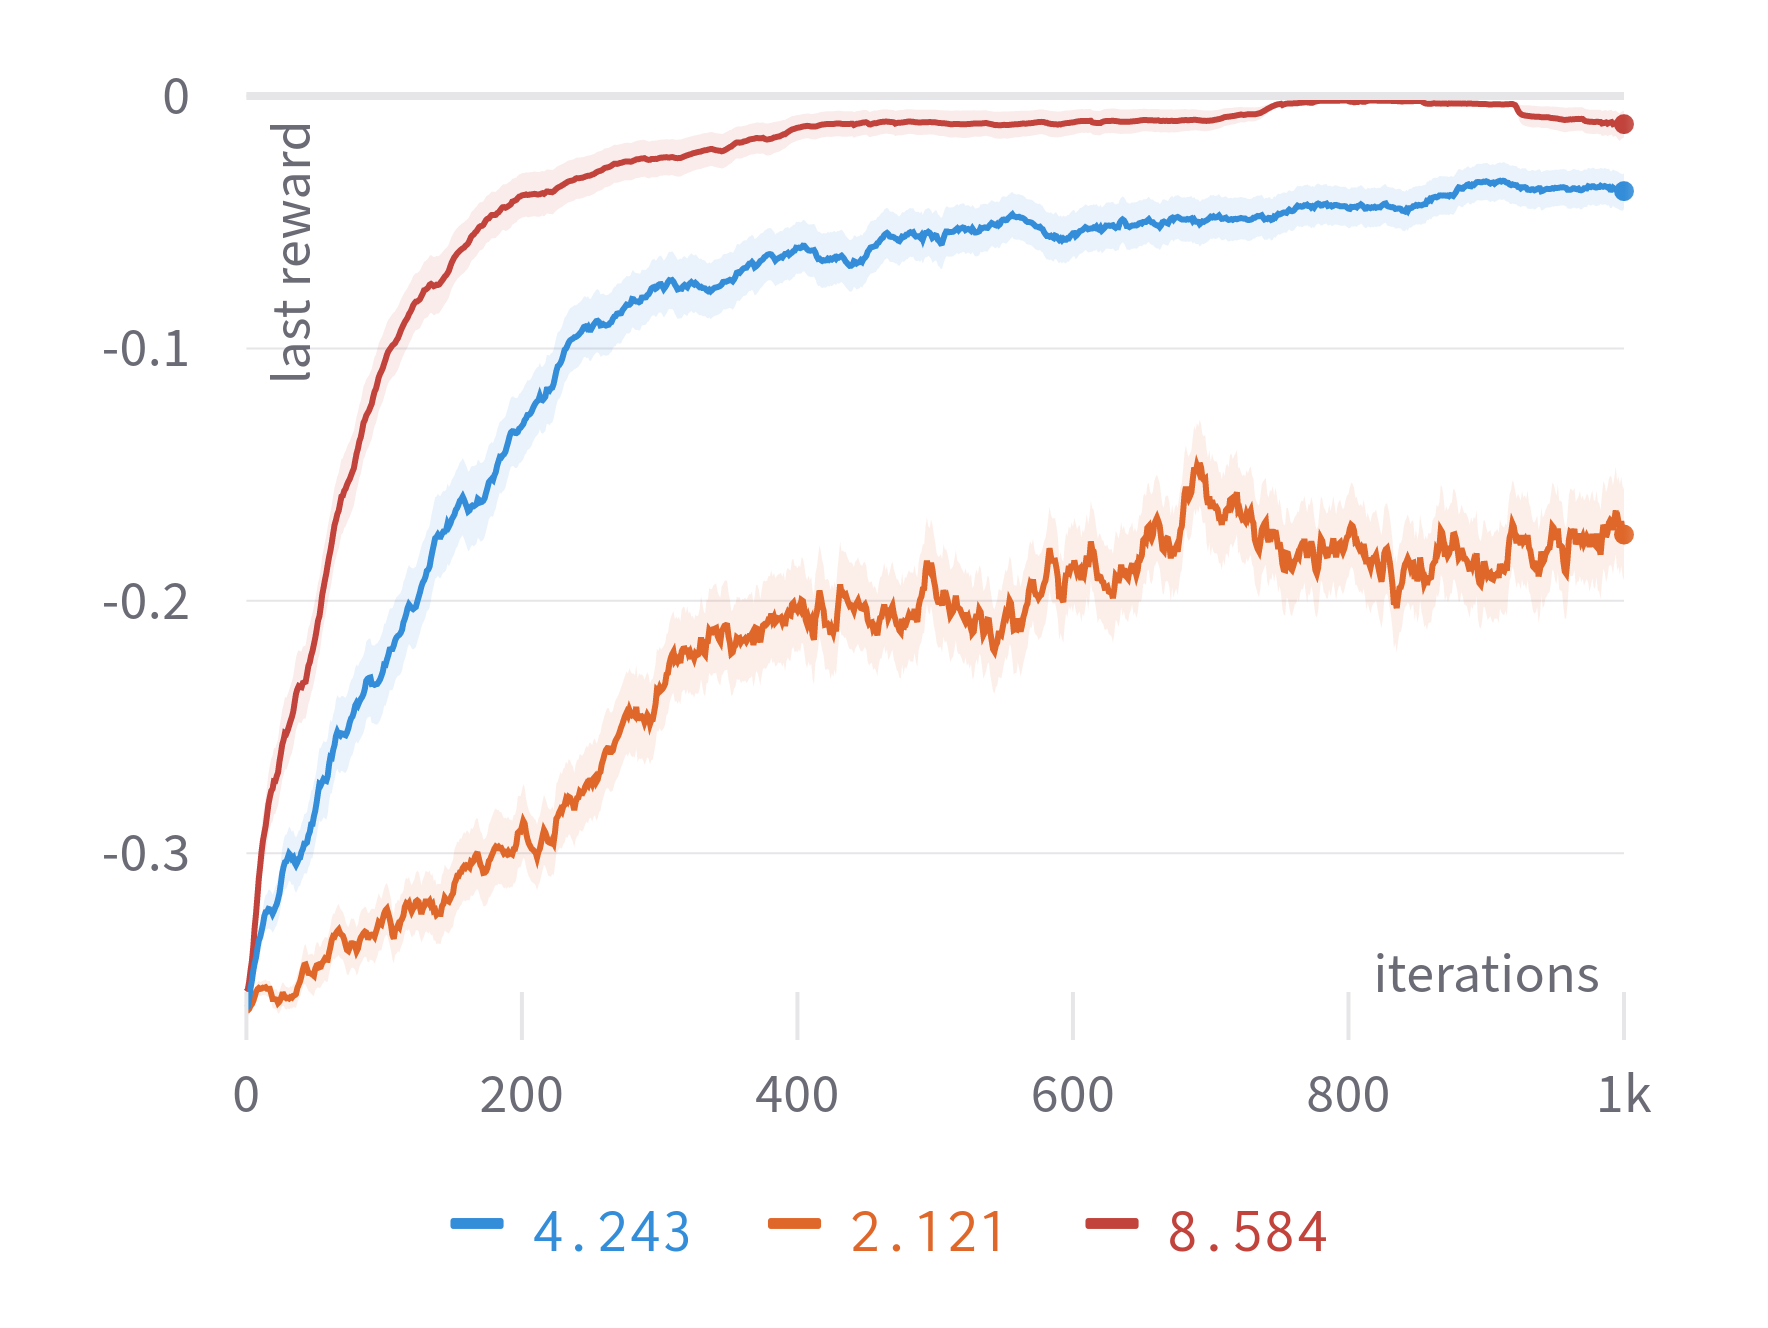
\includegraphics[width=0.49\textwidth]{figures/observation_distance.png}}  
    \hspace{1cm}                       
    \caption{Looking at the performance under different observation ranges. The left side shows different number of neighboring agents and the right side shows different observation distances.}
    \label{fig:observation-knnvsdistance}
\end{figure}

\begin{figure}[htp]
    \centering
    \subfigure[kNN, 50$\%$]{\label{fig:observation-knn-example}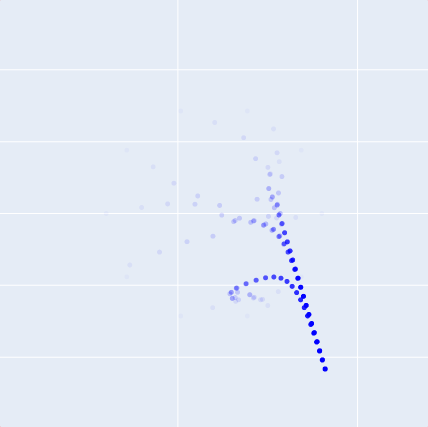
\includegraphics[width=0.40\textwidth]{figures/observation_knn_example_50perc.png}}  
    \subfigure[Euclidean, 12.5$\%$]{\label{fig:observation-distance-example}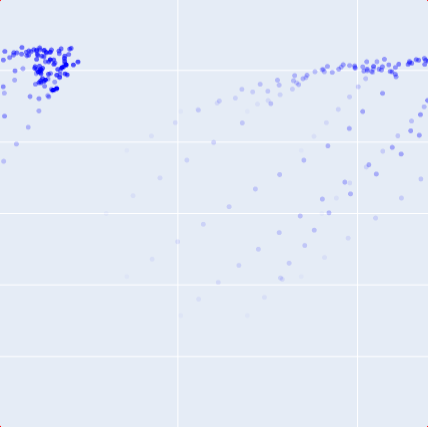
\includegraphics[width=0.40\textwidth]{figures/observation_distance_example_12_5perc.png}}  
    \hspace{1cm}                       
    \caption{Two example episodes.}
    \label{fig:observation-examples}
\end{figure}

The first \Cref{fig:observation-knnvsdistance} shows that in general, the architecture struggled a lot with learning kNN culling. The Euclidean distance is symmetrical, if a sees b then b sees a. but kNN is highly asymmetrical. This leads to a directed graph between agents. So, information flow is very restricted and even incomplete locally. Some observations might never reach parts of the agents. The example episodes shown in \Cref{fig:observation-examples} clearly demonstrate this behavior. It demonstrates how the agents converge on local groups first followed by each group trying the find the other groups and converging globally. This breaks for small k in kNN. For 12.5$\%$ and 25$\%$ culling in kNN, no learning was achieved.


\begin{figure}[htp]
    \centering
    \subfigure[25 $\%$ Distance, Latent Dimension of 8]{\label{fig:observation-dist-25perc}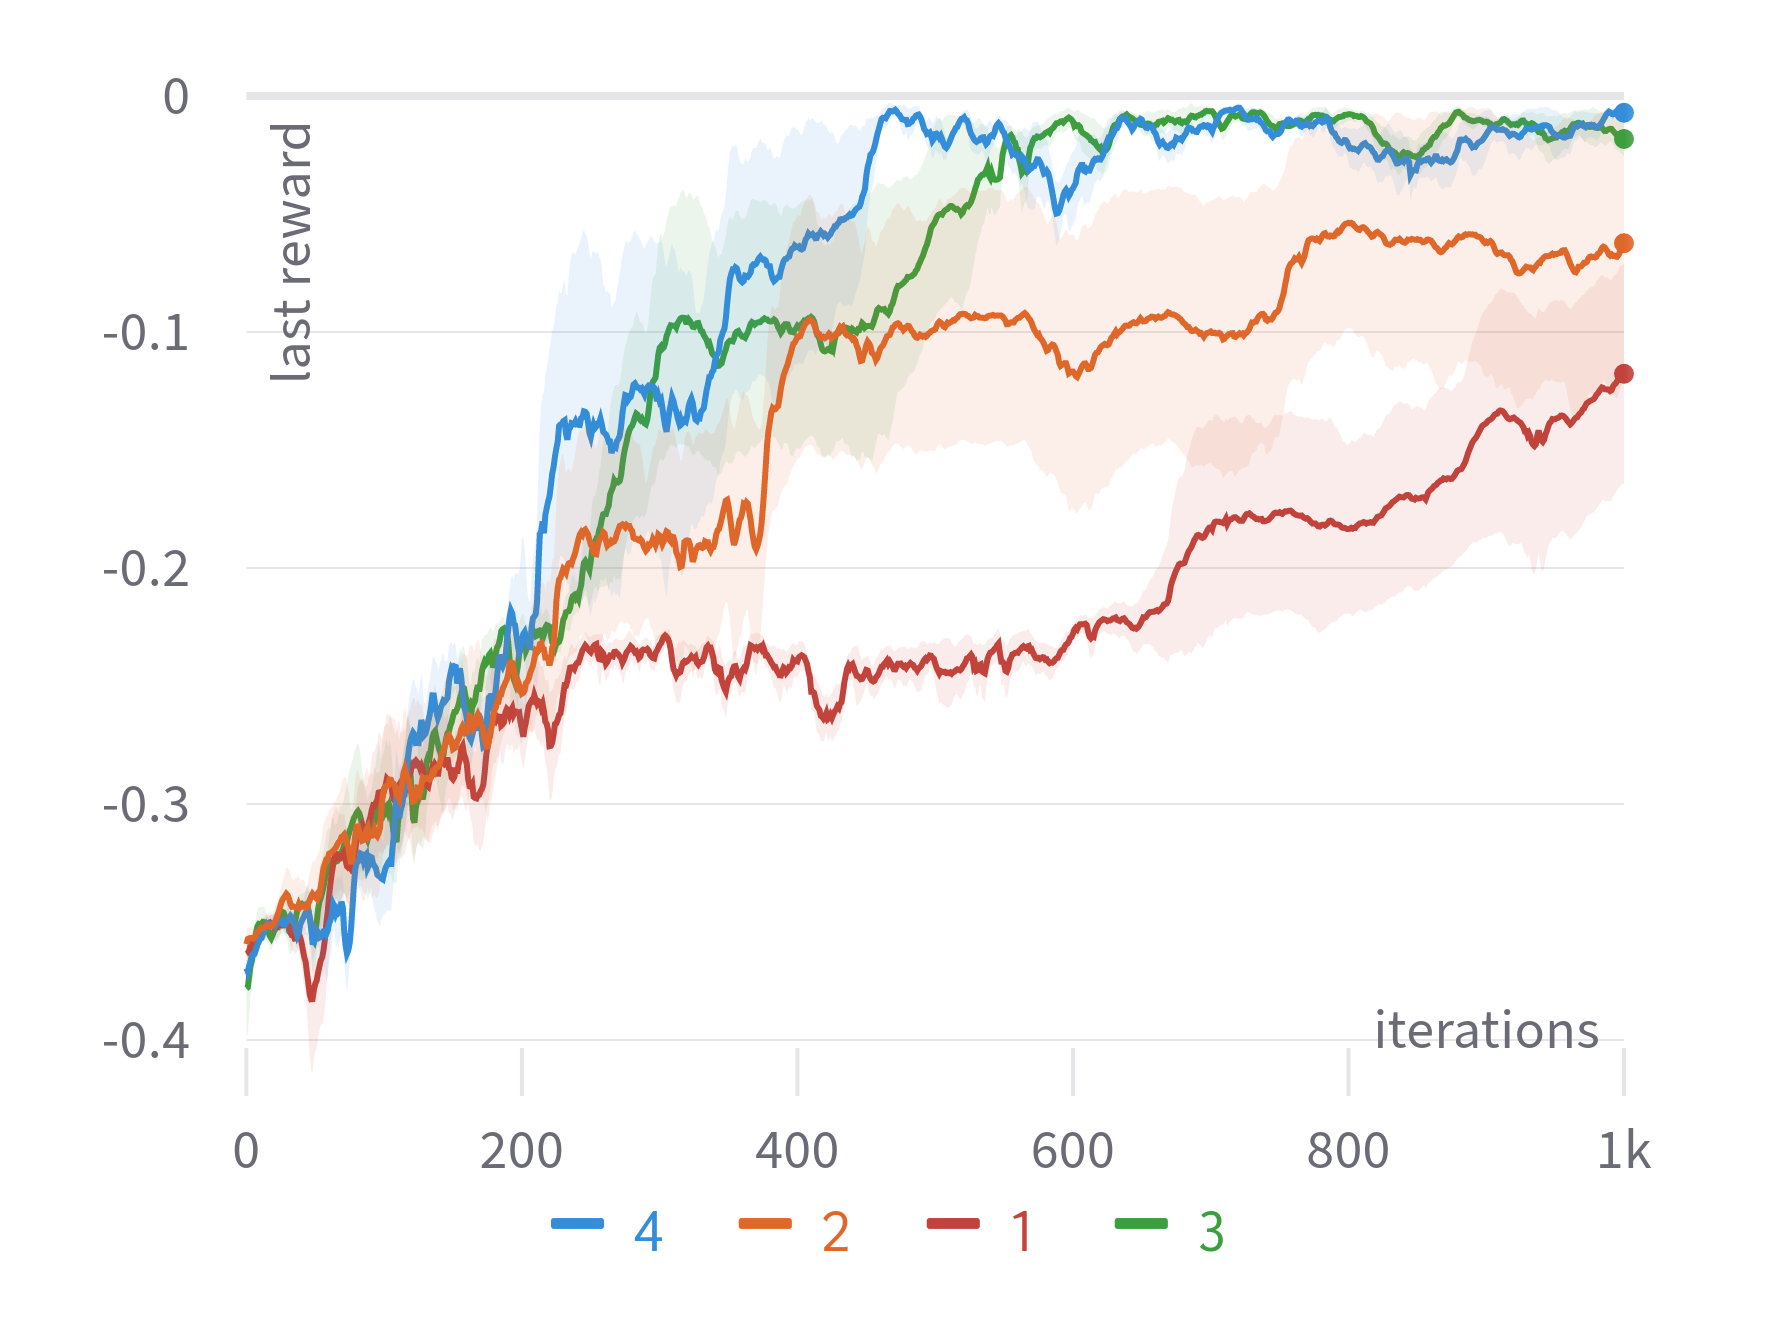
\includegraphics[width=0.49\textwidth]{figures/observation_distance_25perc_ld8.png}}  
    \subfigure[12.5 $\%$ Distance]{\label{fig:observation-dist_12_5perc}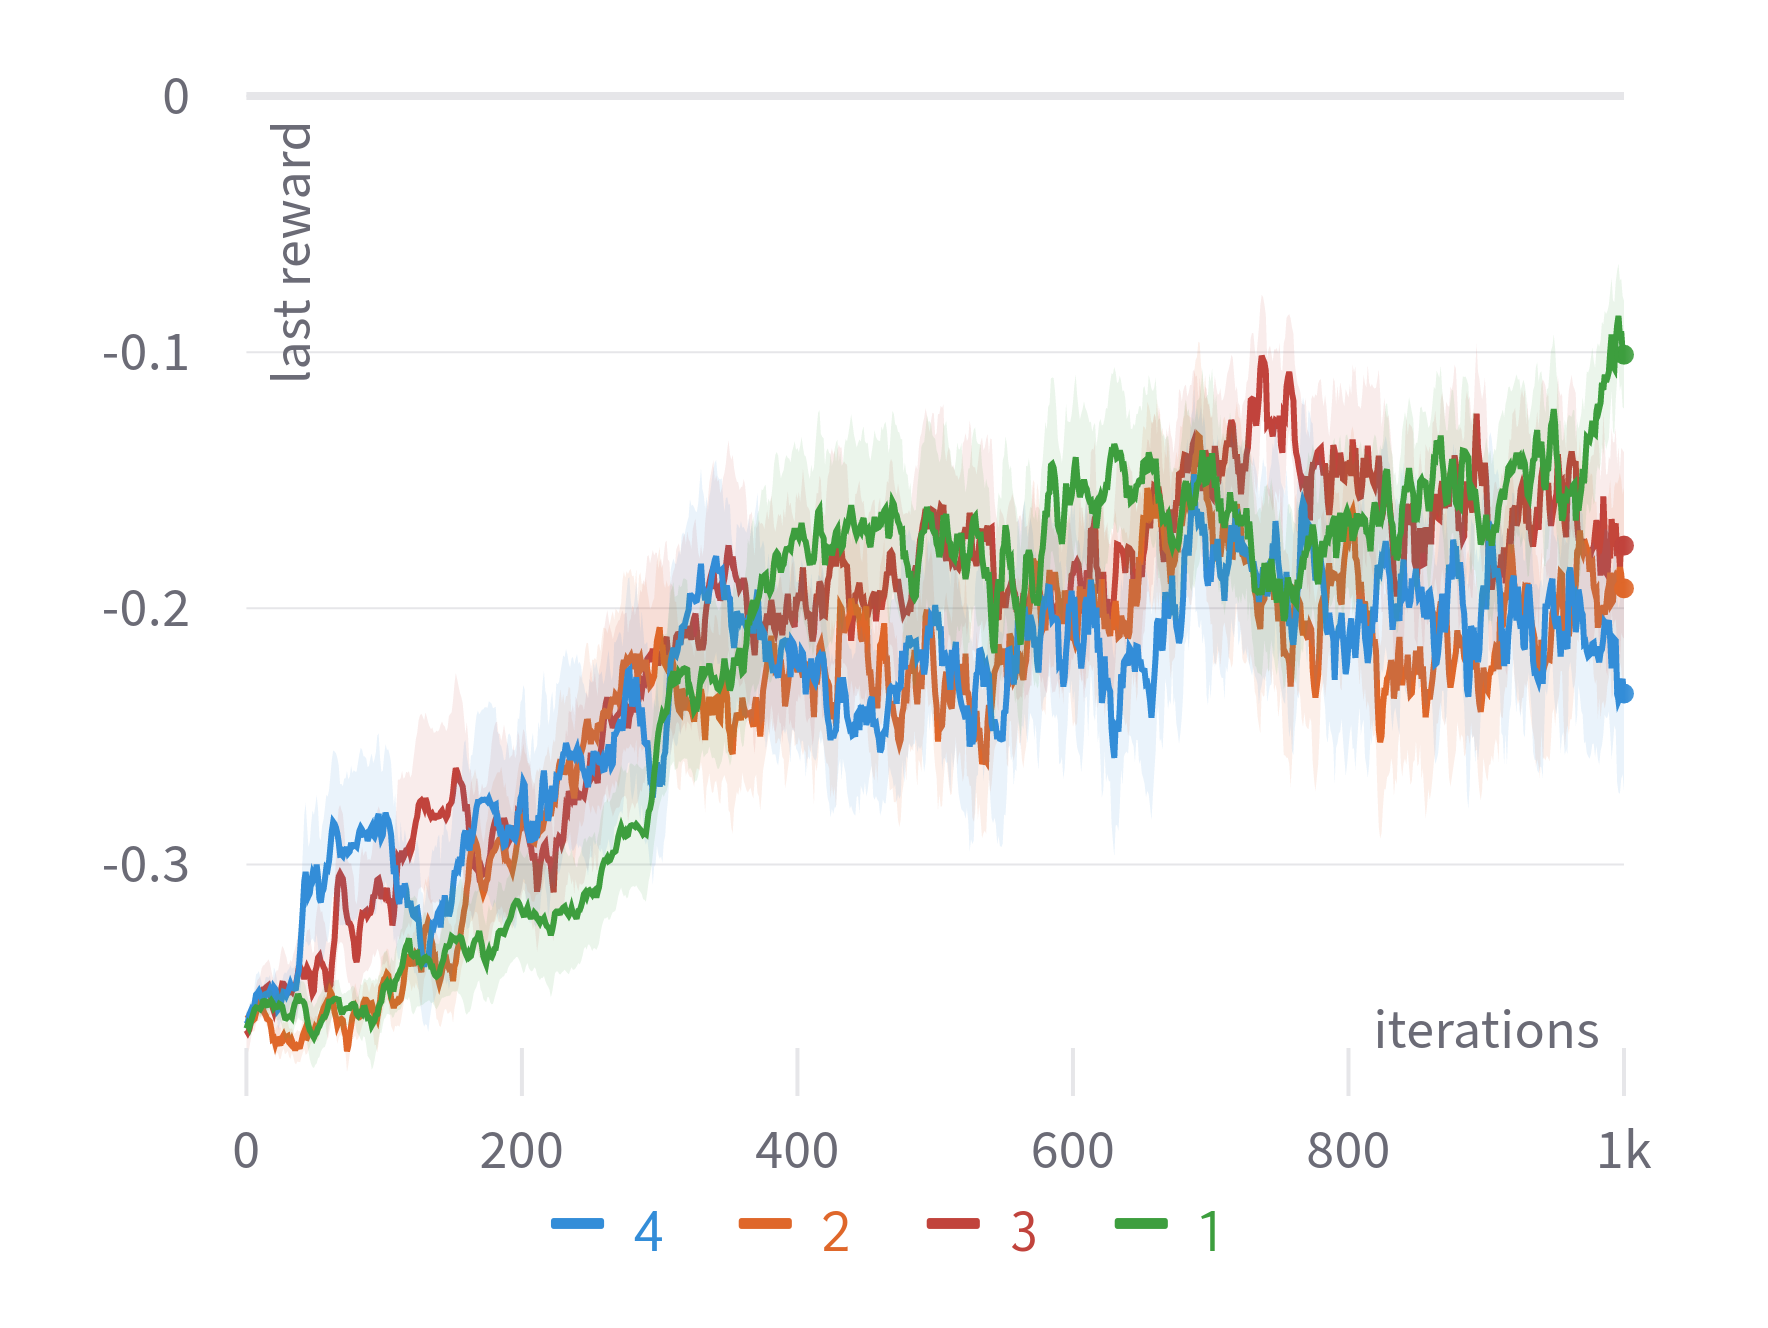
\includegraphics[width=0.49\textwidth]{figures/observation_distance_12_5perc.png}}  
    \hspace{1cm}                       
    \caption{Comparison of 25$\%$ and 12.5 $\%$ distance culling for different number of GNN hops.}
    \label{fig:observation-distancecompare}
\end{figure}

For distance culling, 50$\%$ was generally not different than our proof of concept. This might be because of our specific evaluation setup. The agents always spawn in a circle with the radius being half the world size. 50$\%$ is just enough so that each agent can see each other.
In \Cref{fig:observation-distancecompare} we examined distance culling in a little bit more detail. The right side shows that the number of hops did not make a difference, as the architecture struggled to learn under these constraints. For 25$\%$, which is shown on the left side, we observed large differences between the number of hops for a latent dimension of 8. For higher latent dimension this was still the case, but not as pronounced. This seems to suggest that if the constraints are even more severe and the task itself is solvable for the number of iterations provided, the gain for multiple GNN Hops is large. Though with more than 3 hops, no real benefit is shown.


\section{Pursuit Results}
We originally intended to also run our experiments on the Pursuit environment. This included observation tests and examining both heterogeneous aggregation types. We hoped that a more complex task could lead to even more pronounced evidence for the advantage of multiple GNN Hops. Unfortunately, due to the aforementioned hardware issues and time constraints, we were not able to produce adequate results. We found that even simple Single-Evader Pursuit test cases oscillated heavily. We tried running multiple experiments with increasing difficulty. Our investigations showed, that when the evader has a randomized starting position, the experiments break. Even with extensive debugging we were not able to find a logical or mathematical error in either the environment itself or the heterogeneous graphs. We additionally tried to extend our architecture with one MLP per Node-, or Edge-Type in the heterogeneous modules. This showed a more stable solution in the resulting policy, which still did not learn the task at hand. At the point of writing, it is unclear if the problem exists within our implementation of the environment or the heterogeneous GNN.


\iffalse
\section{Neighbor Aggregation Types}
\label{sec:Neighbor Aggregation Types}
Which environments used and special setting, (grid)
\begin{itemize}[noitemsep,nolistsep]
    \item Environments: Pursuit-Single, Pursuit-Multi
    \item Environment: Base-Pursuit-Multi with 3+ Hops?
    \item Network: latent dimension, aggregation-function, neighbor-aggregation (aggr(aggr()) vs concat(aggr())), num-blocks
\end{itemize}
Questions to answer:
\begin{itemize}[noitemsep,nolistsep]
    \item Agents better/worse being able to distinguish themselves from evaders for concat(aggr())?
    \item How does this effect aggregation function for aggr(aggr()). Where do I get better performance?
    \item How is the effect of more/less hopps here?
\end{itemize}
(Expected) Result:
\begin{itemize}[noitemsep,nolistsep]
    \item concat(aggr()): worse iteration time, but easier to learn heterogeneous graphs.
    \item aggr(aggr()): probably mean aggregation, there are more features "preserved".
    \item num-hops: more hops should have more of an effect in concat(aggr()).
\end{itemize}


\section{Directed vs Undirected GNN}
\label{sec:Directed vs Undirected GNN}
Which environments used and special setting, (grid)
\begin{itemize}[noitemsep,nolistsep]
    \item Environments: Pursuit-Multi, Pursuit-Single
    \item Just add this to each of the other experiments (?)
    \item Environements: use-directed-graph.
    \item Network: num-blocks, latent dimension, aggregation-function, neighbor-aggregation, value-function-scope
\end{itemize}
Questions to answer:
\begin{itemize}[noitemsep,nolistsep]
    \item what "learns" better or has better information propagation
\end{itemize}
(Expected) Result:
\begin{itemize}[noitemsep,nolistsep]
    \item 
\end{itemize}


\section{Node-wise vs Graph-wise Value-function}
\label{sec:Node-wise vs Graph-wise Value-function}
Which environments used and special setting, (grid)
\begin{itemize}[noitemsep,nolistsep]
    \item Environments: Rendezvous, Pursuit-Single
    \item Just add this to each of the other experiments (?)
    \item Environements: 
    \item Network: num-blocks, latent dimension, aggregation-function, neighbor-aggregation, value-function-scope
\end{itemize}
Questions to answer:
\begin{itemize}[noitemsep,nolistsep]
    \item graph-wise: more "true" to the original Single agent RL algorithms. Should correlate better? But need to figure out themselves which agent is responsible for a reward.
    \item node-wise: better able to to gauge which agent was responsible for a given value or reward. 
\end{itemize}
(Expected) Result:
\begin{itemize}[noitemsep,nolistsep]
    \item 
\end{itemize}
\fi